\chapter{CONCLUSION AND ANALYSIS}
\section{Conclusion}
LabXplorerX is an innovative virtual laboratory platform tailored for enhancing science education through interactive simulations and experiments. It aims to revolutionize how students and educators engage with scientific concepts by offering a diverse range of features. LabXplorerX facilitates seamless exploration, collaboration, and learning aweb various scientific disciplines. This platform empowers users to conduct experiments, share insights, and leverage sophisticated algorithms to deepen their understanding. Additionally, LabXplorerX integrates advanced reporting capabilities and decision-making tools, enriching the educational experience beyond traditional classroom settings.
\section{Work Completed}

In the LabXplorerX project, significant strides have been made in creating an engaging and educational platform for students. The development team has successfully accomplished the following key tasks:

\begin{itemize}[leftmargin=1cm]
    \item \textbf{Creation of Simulations:} Successfully developed 5 interactive simulations, including the Gravity Simulator, Ohm's Law Simulator, Atom Simulator, Solar System Simulator, and JavaScript Editor, each tailored to provide hands-on learning experiences across various subjects.
    
    \item \textbf{Learning Capsules:} Created comprehensive learning capsules that include structured content, interactive elements, and visual aids to enhance student understanding. These capsules cover various educational categories and provide multimedia-rich content.
    
    \item \textbf{Authentication:} Implemented a robust authentication system to manage user access, including secure login, registration, and account management features for both students and teachers.
    
    \item \textbf{Admin Panel:} Developed an admin panel that allows administrators to efficiently manage users, simulations, and content. The panel includes tools for monitoring user progress, updating content, and overseeing the overall platform.
    
    \item \textbf{Quizzes:} Integrated quizzes into the learning modules, enabling students to assess their understanding of the material. The quizzes are designed to be interactive and provide immediate feedback to the learners.
    
    \item \textbf{User Interface Screens:} Developed various user interface screens such as the Home Screen, Login Screen, Register Screen, About Page, Learning Areas Screen, Simulations Screen, and more. Each screen has been documented with corresponding screenshots to showcase the user experience.
\end{itemize}

All planned features have been successfully implemented, and the platform is now equipped with interactive simulations, structured learning capsules, secure authentication, comprehensive admin tools, and engaging quizzes.
\newpage
\subsection{Screenshots of Outcomes}
% Home Screen
\textbf{Home Screen:} Below is the screenshot of the Home Screen, which is the main interface of the application.
\begin{figure}[H]
    \centering
    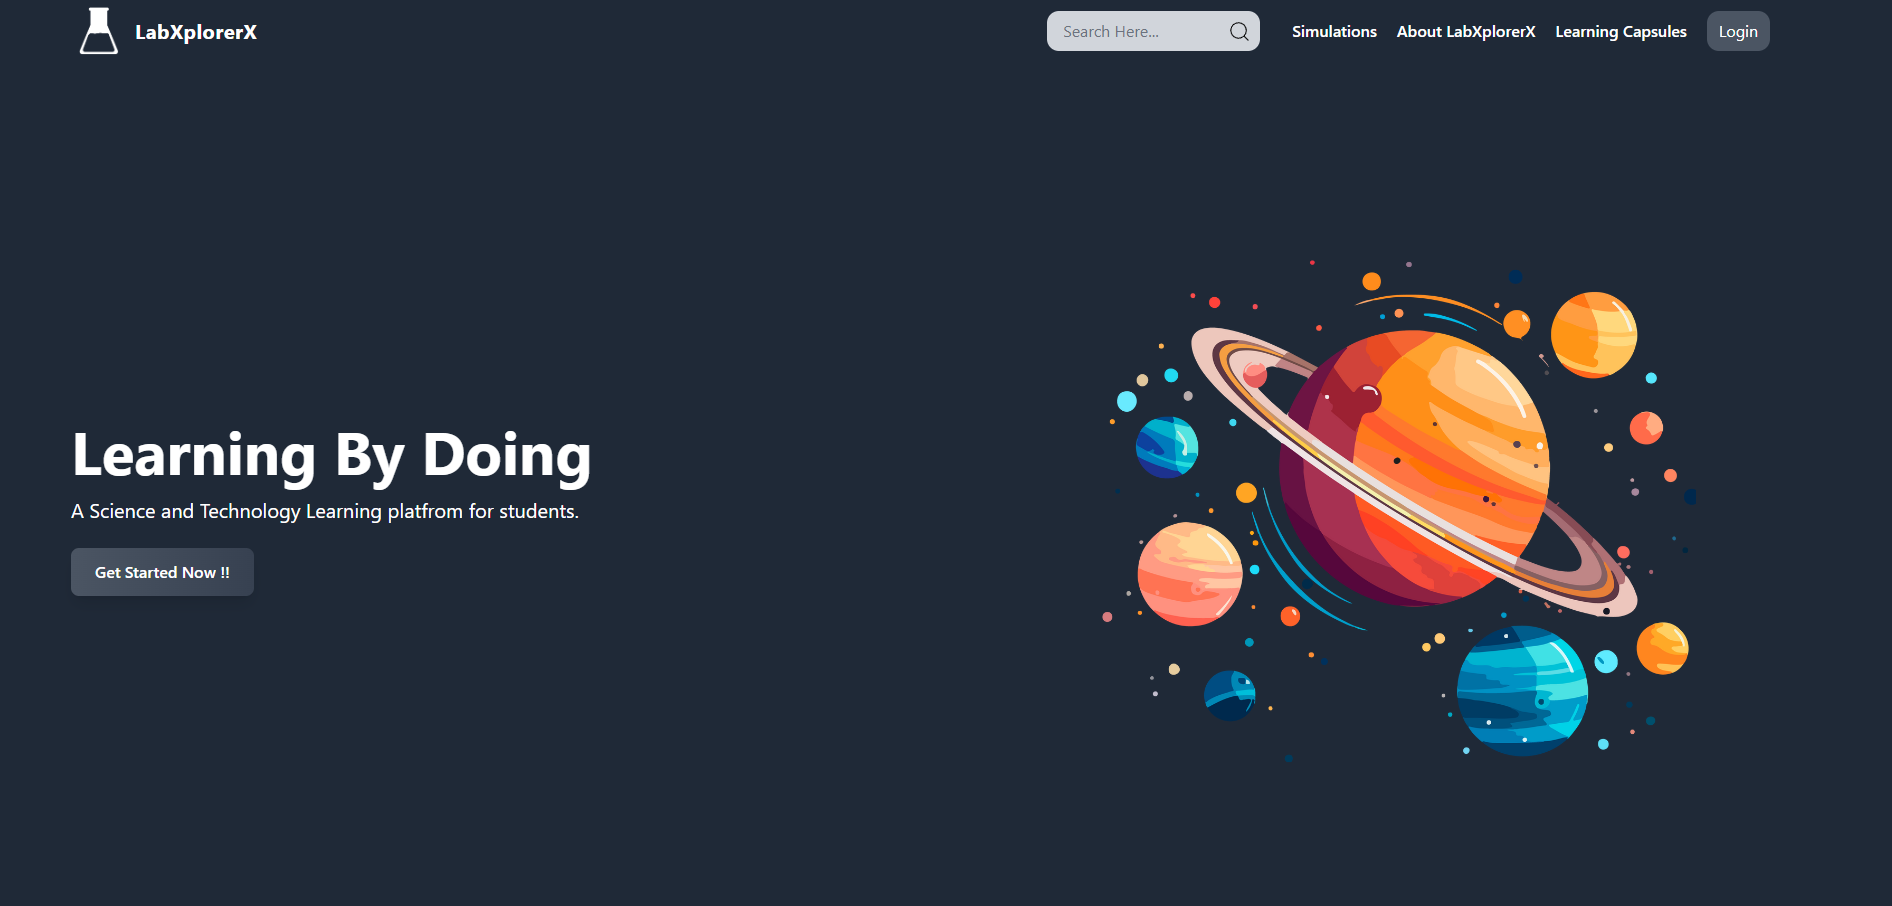
\includegraphics[width = 14cm]{Diagrams/output/home.png}
    \caption{Home Screen}
\end{figure}

% Login Screen
\textbf{Login Screen:} Below is the screenshot of the Login Screen, where users enter their credentials to access their accounts.
\begin{figure}[H]
    \centering
    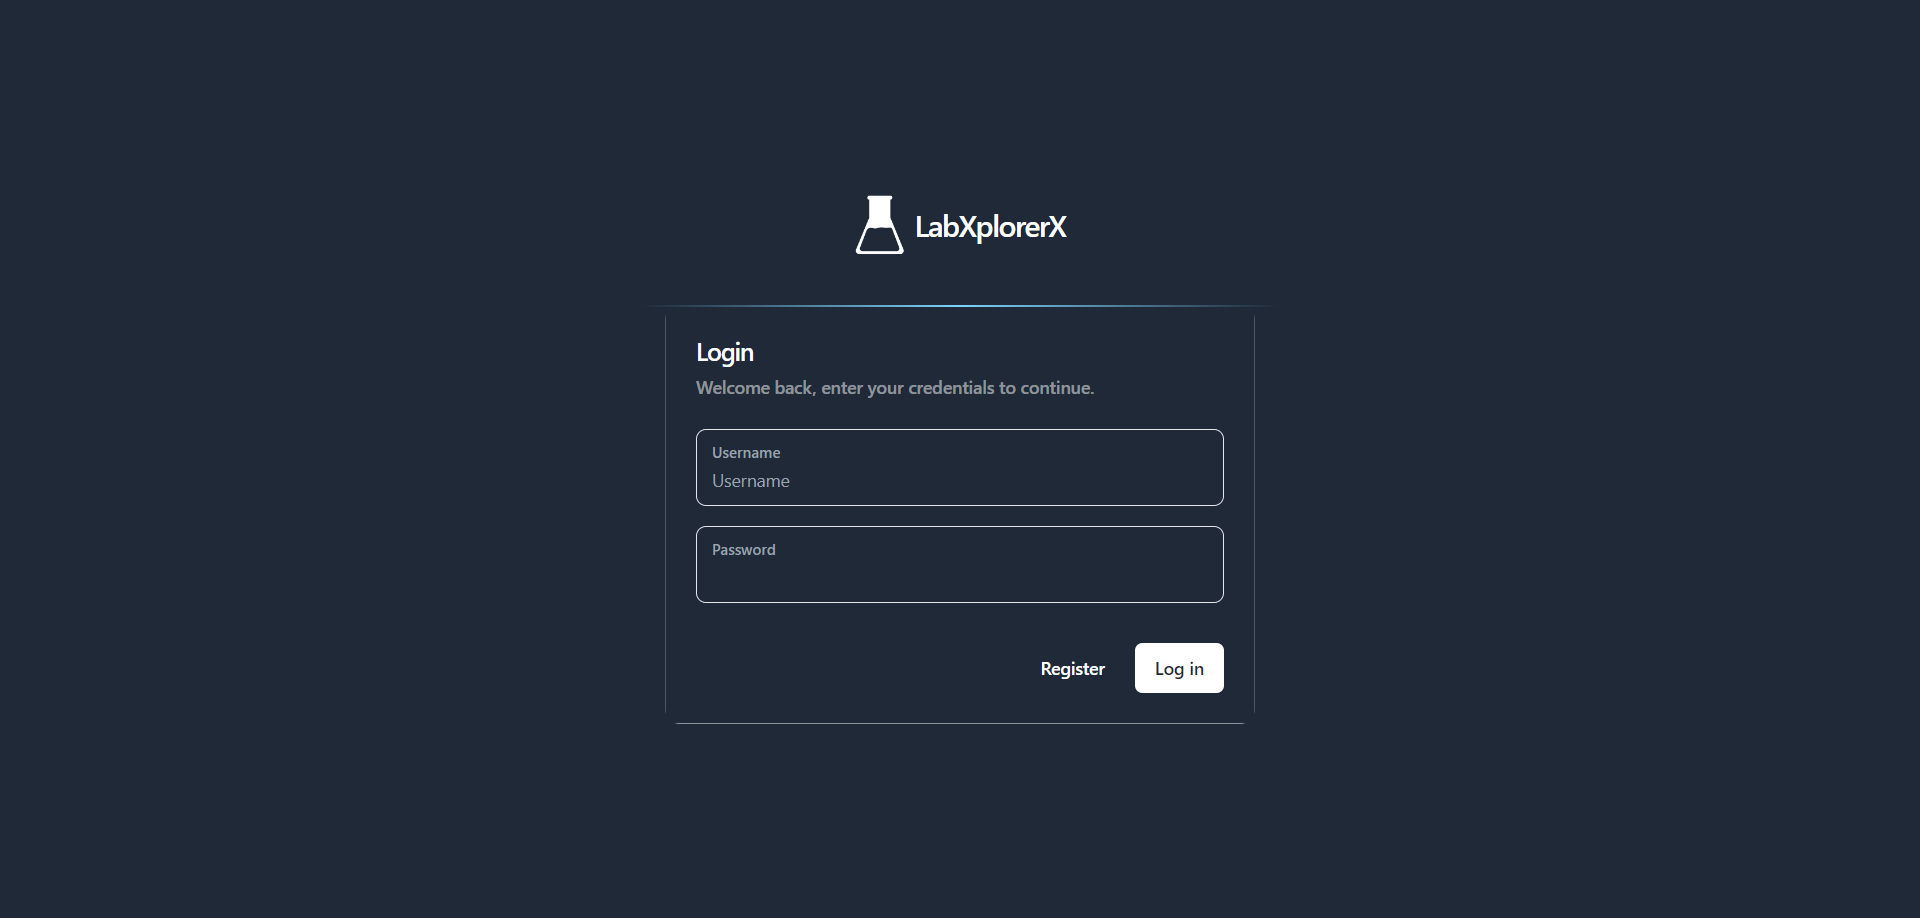
\includegraphics[width = 15cm]{Diagrams/output/login.png}
    \caption{Login}
\end{figure}
\newpage
% Register Screen
\textbf{Register Screen:} Below is the screenshot of the Register Screen, where new users can create an account.
\begin{figure}[H]
    \centering
    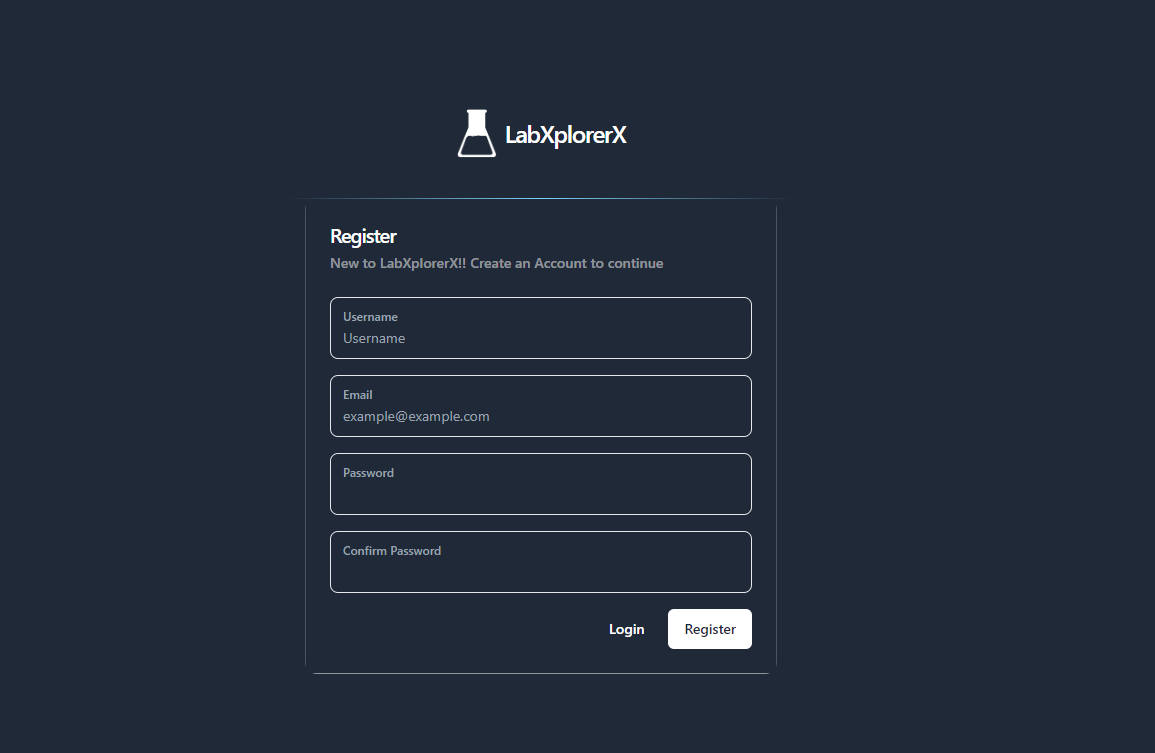
\includegraphics[width = 16cm]{Diagrams/output/register.png}
    \caption{Register}
\end{figure}

% About Page
\textbf{About Page:} Below is the screenshot of the About Page, which provides information about the application.
\begin{figure}[H]
    \centering
    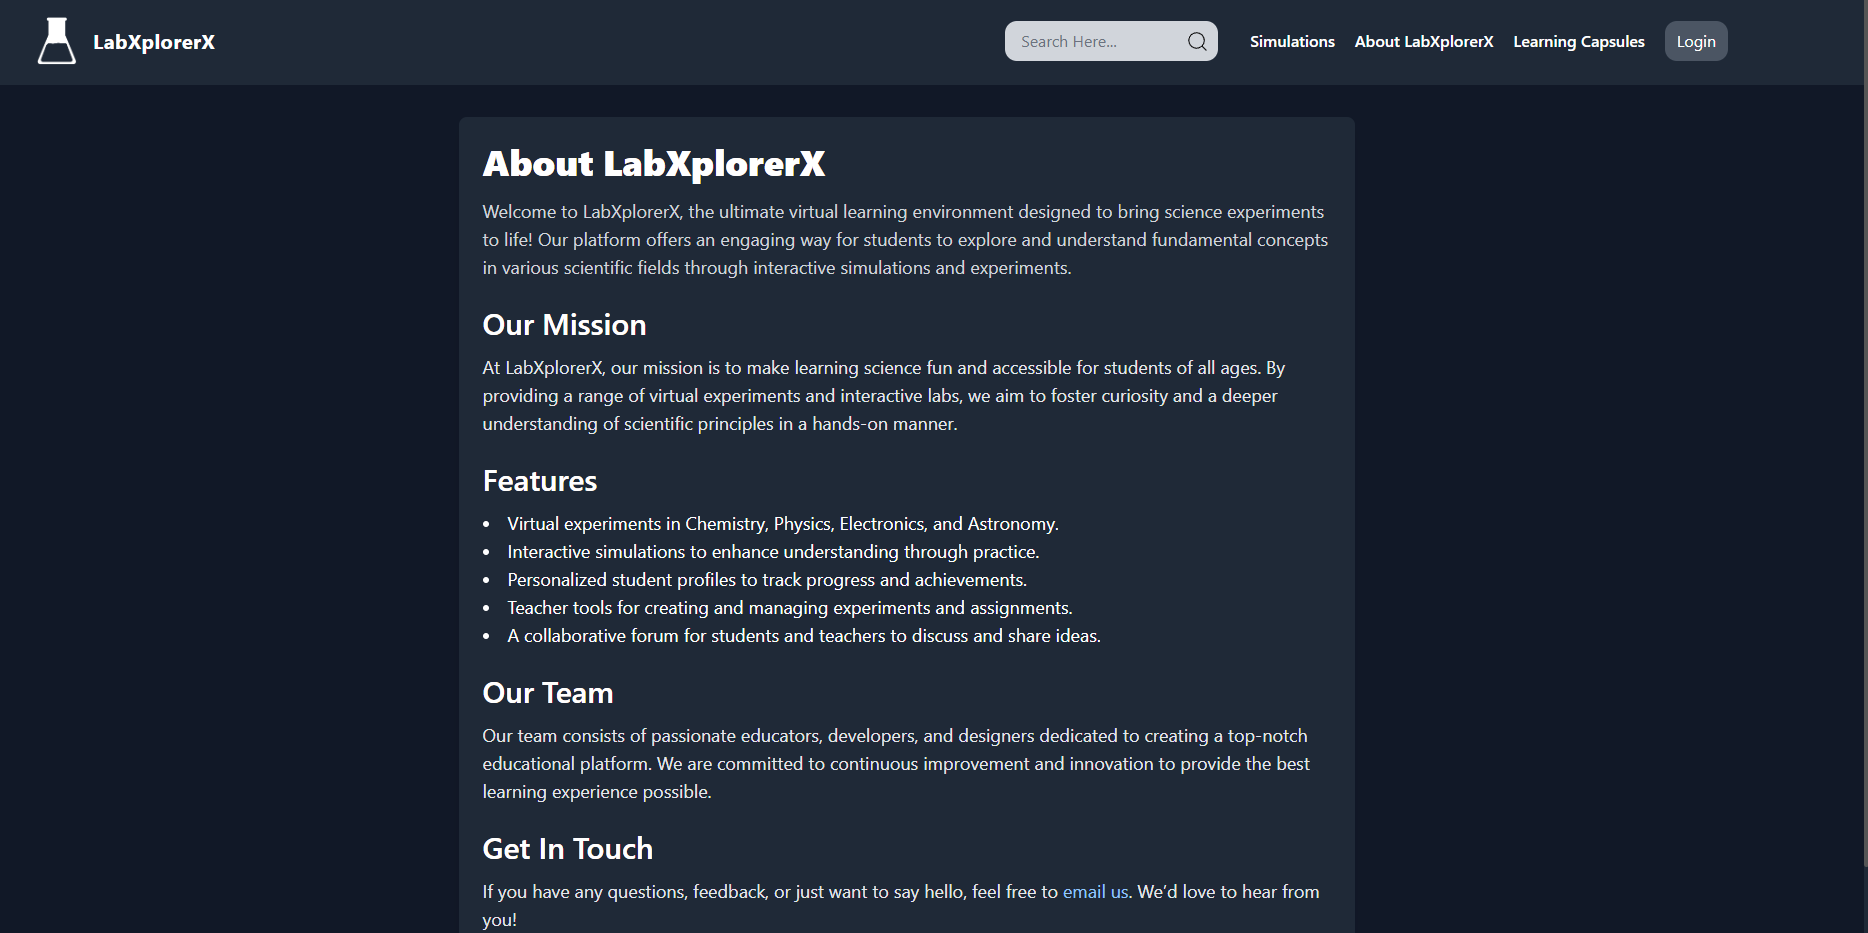
\includegraphics[width = 16cm]{Diagrams/output/about.png}
    \caption{About Page}
\end{figure}
\newpage

% Learning Areas Screen
\textbf{Learning Areas Screen:} Below is the screenshot of the Learning Areas Screen, showing the various educational categories available.
\begin{figure}[H]
    \centering
    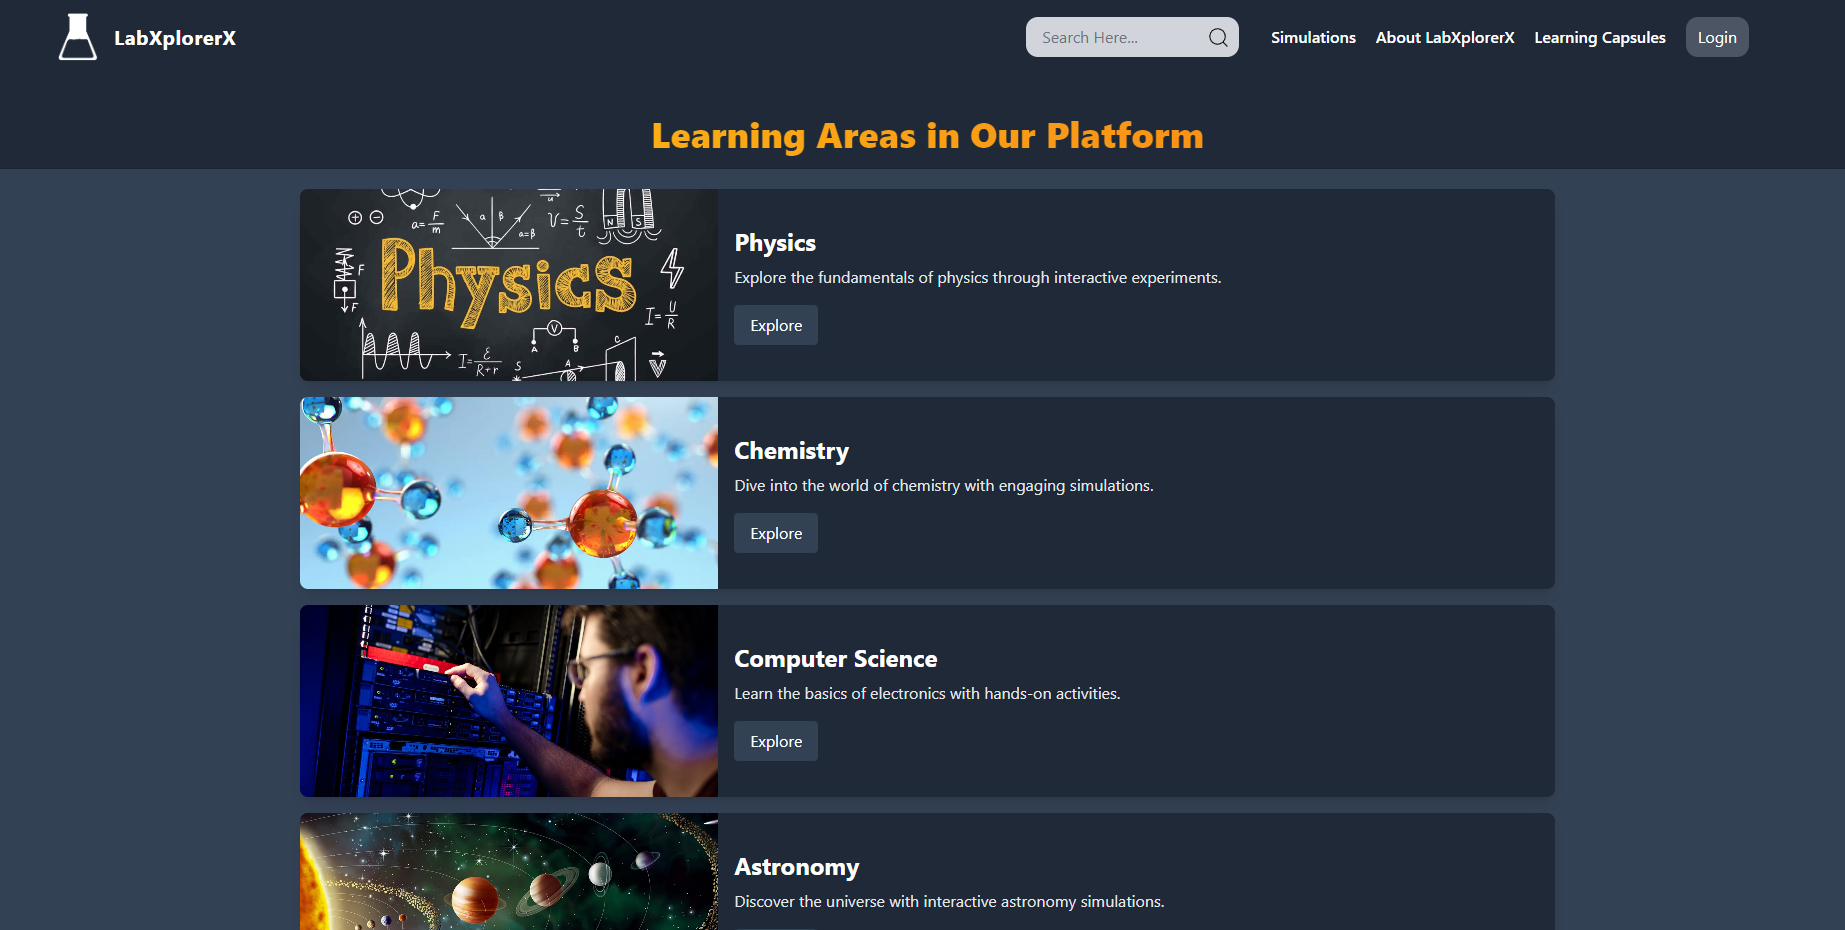
\includegraphics[width = 15cm]{Diagrams/output/learningareas.png}
    \caption{Learning Areas}
\end{figure}

% Simulations Screen
\textbf{Simulations Screen:} Below is the screenshot of the Simulations Screen, where users can access different simulations.
\begin{figure}[H]
    \centering
    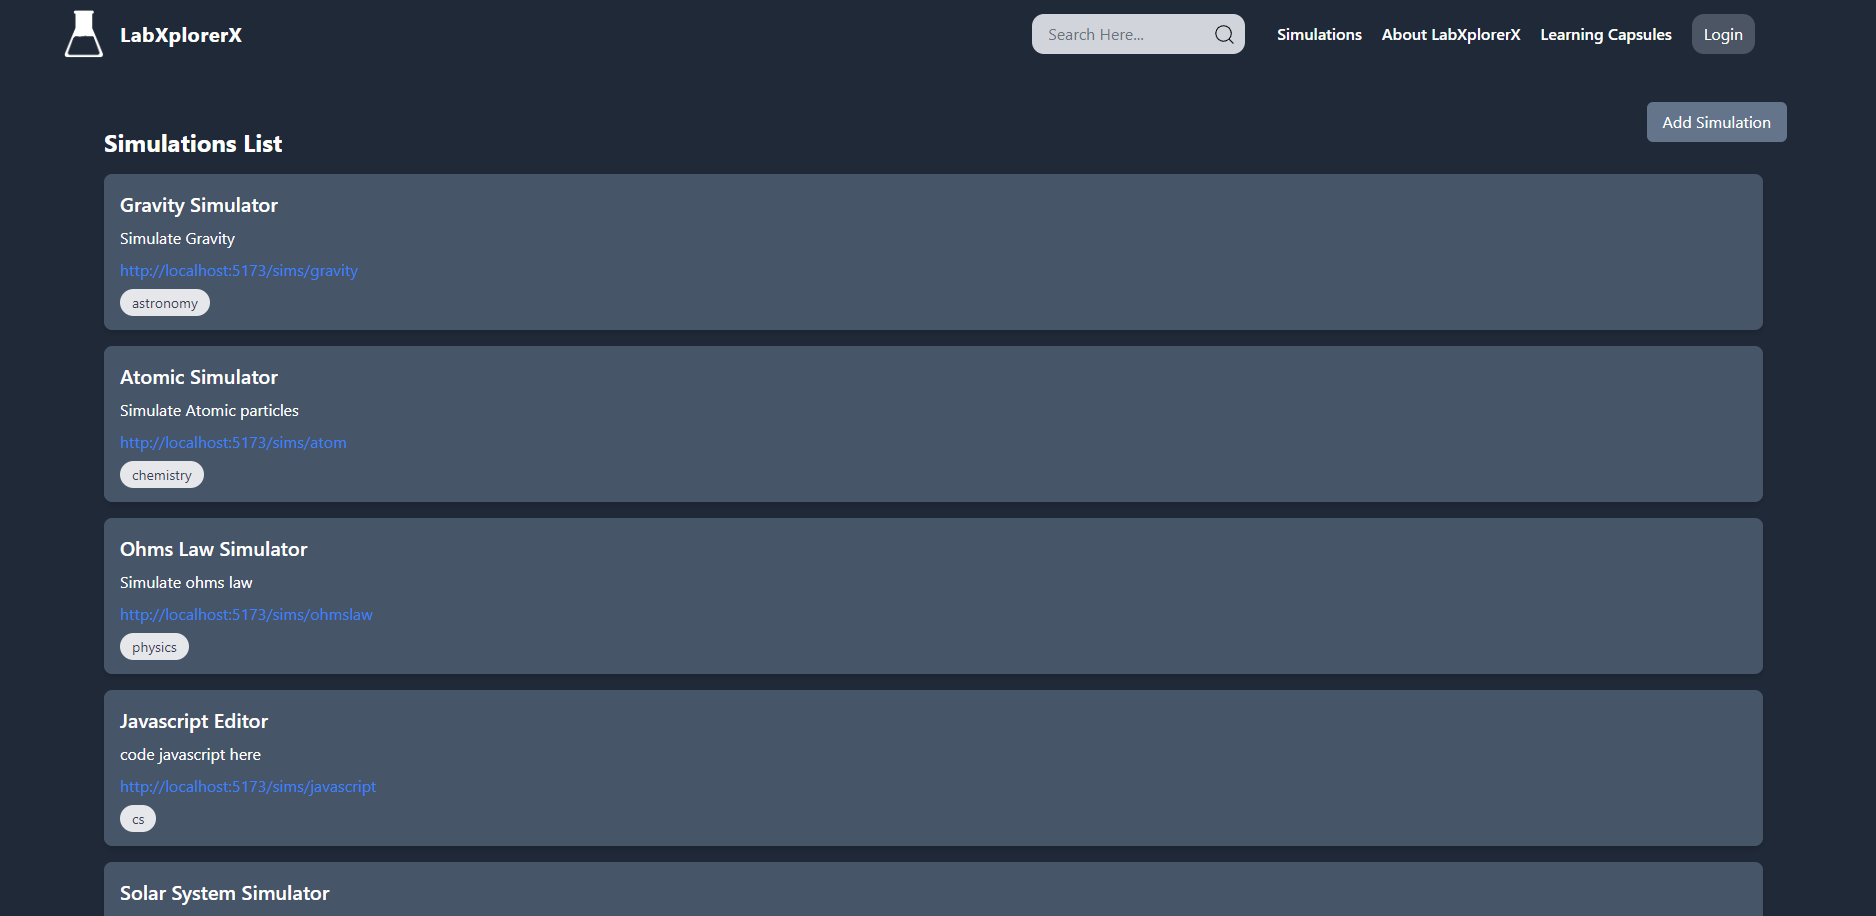
\includegraphics[width = 15cm]{Diagrams/output/simulations.png}
    \caption{Simulations}
\end{figure}

% Capsules Screen
\textbf{Capsules Screen:} Below is the screenshot of the Capsules Screen, which displays the available capsules in the application.
\begin{figure}[H]
    \centering
    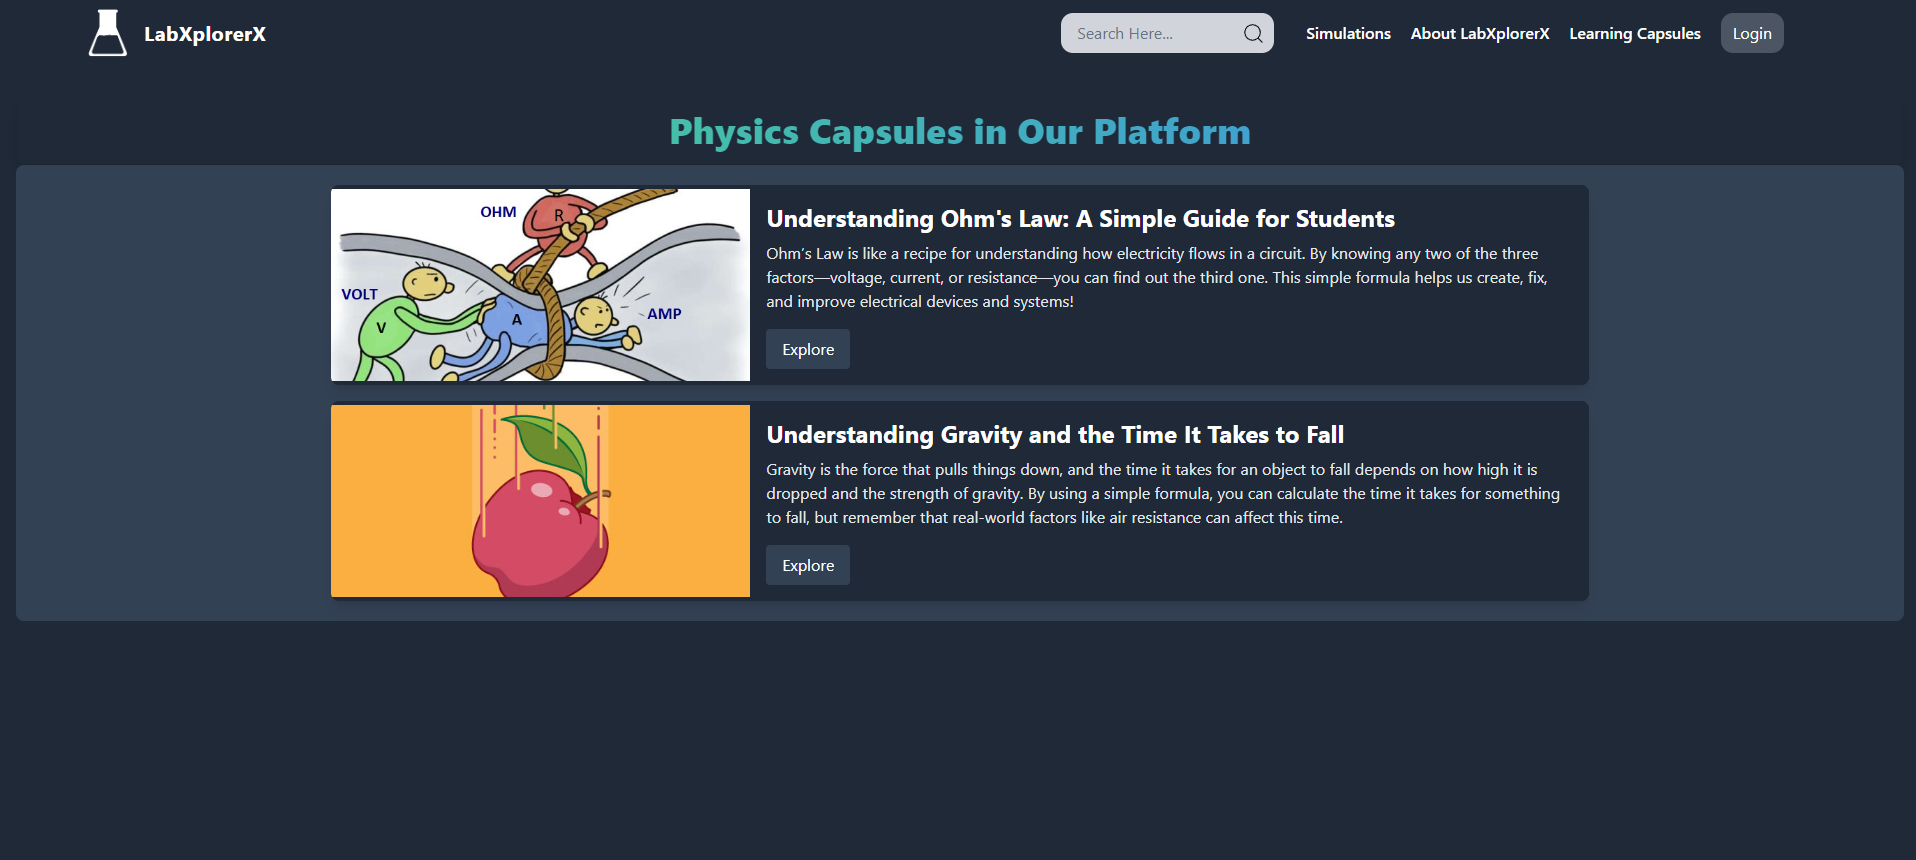
\includegraphics[width = 16cm]{Diagrams/output/capsules.png}
    \caption{Capsules}
\end{figure}

% Quizzes Screen
\textbf{Quizzes Screen:} Below is the screenshot of the Quizzes Screen, where users can participate in various quizzes.
\begin{figure}[H]
    \centering
    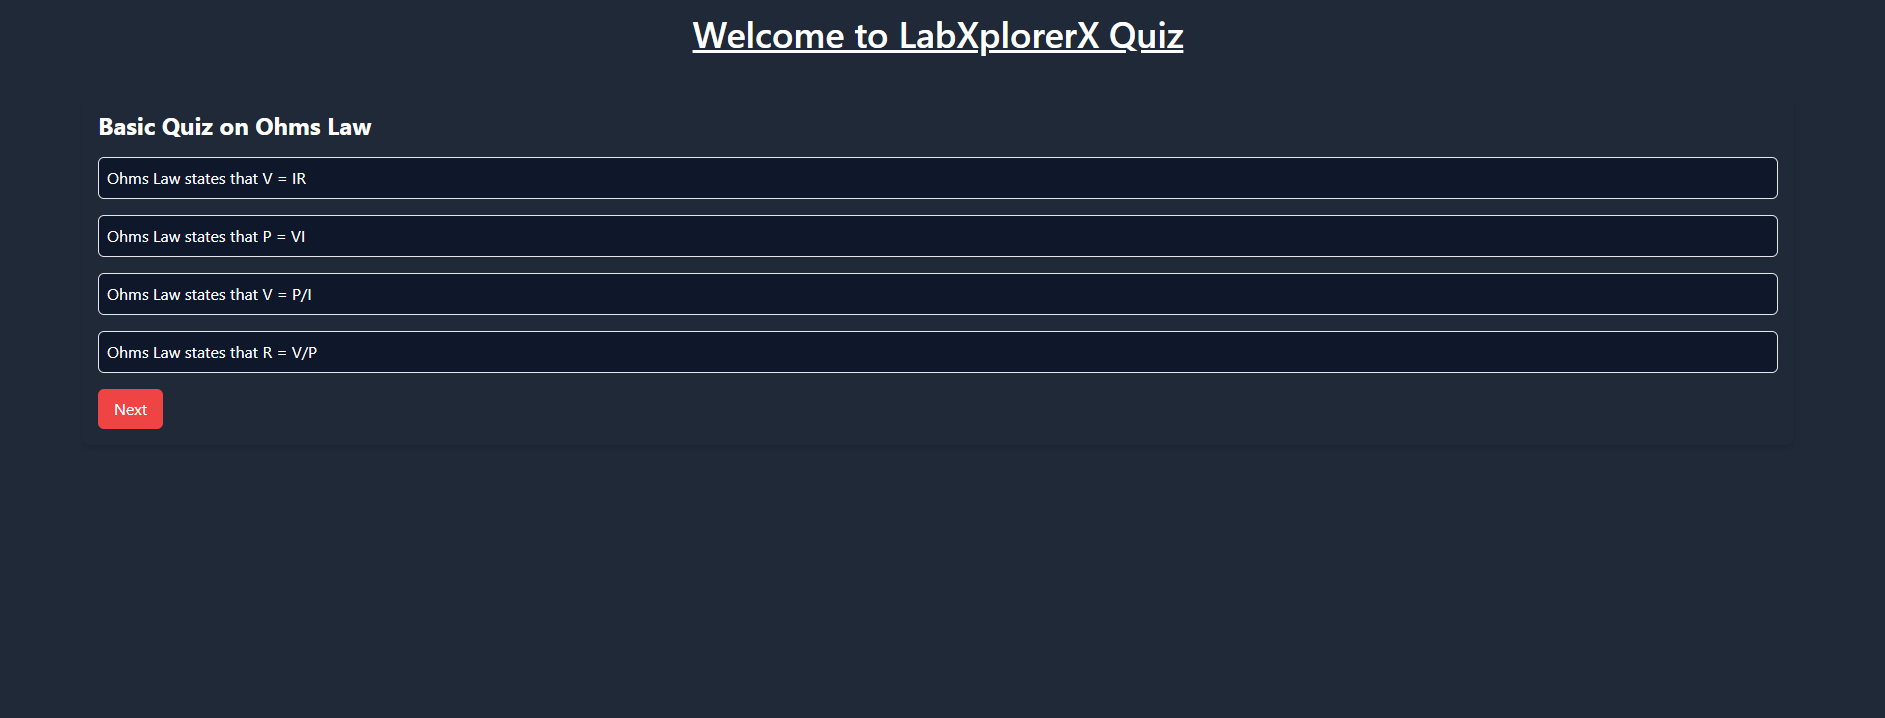
\includegraphics[width = 16cm]{Diagrams/output/quiz.png}
    \caption{Quizzes}
\end{figure}
\newpage

% Admin Panel
\textbf{Admin Panel:} Below is the screenshot of the Admin Panel, used by administrators to manage the application.
\begin{figure}[H]
    \centering
    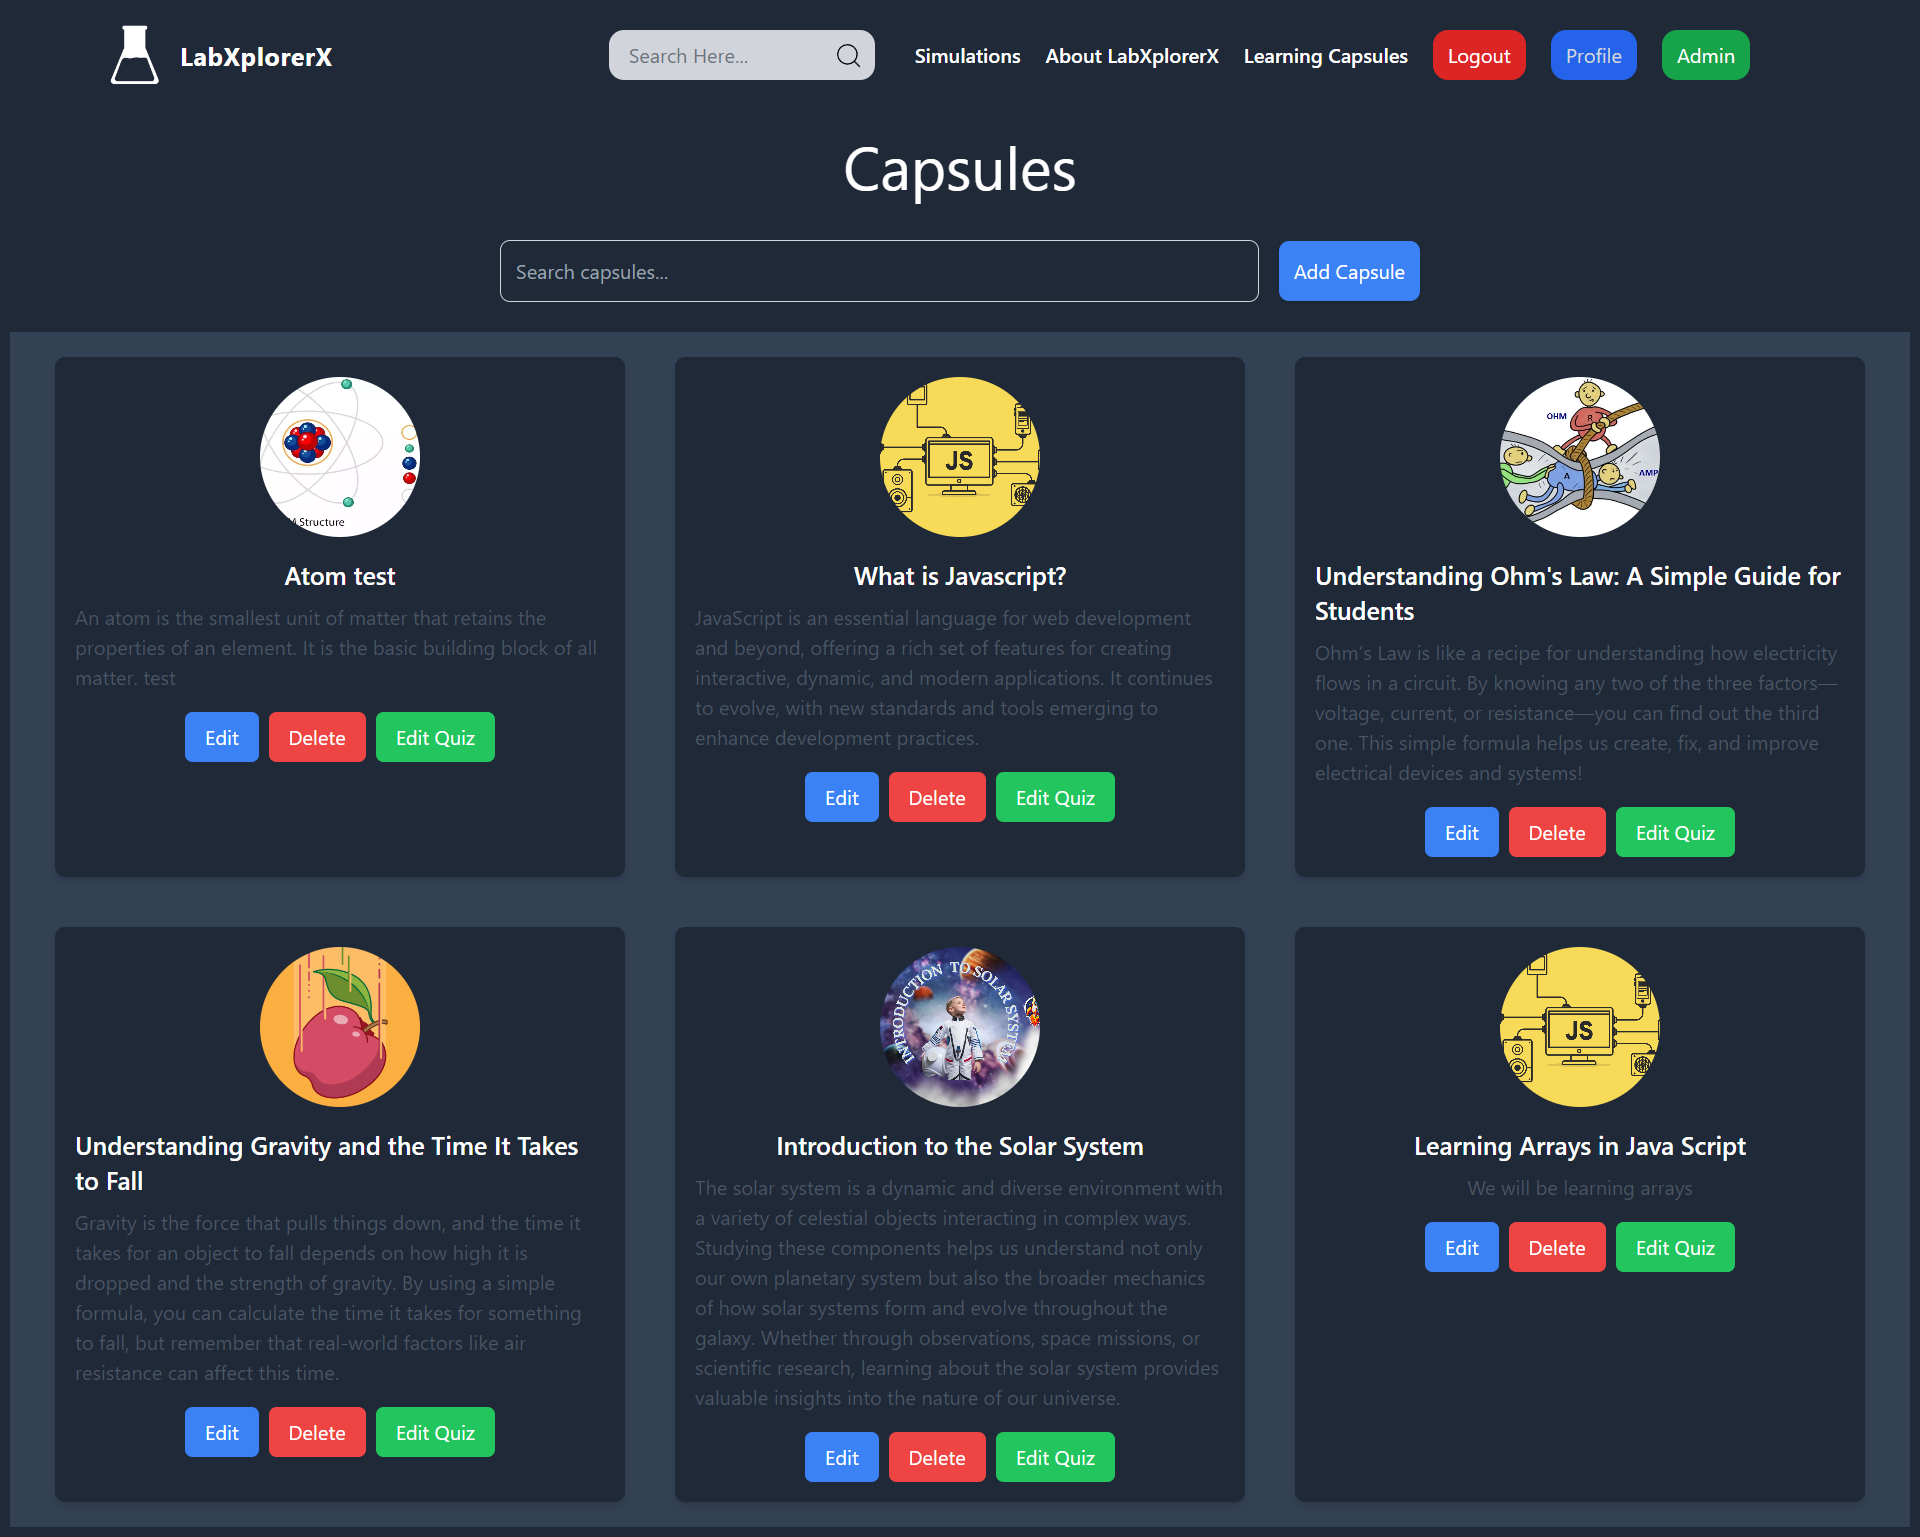
\includegraphics[width = 16cm]{Diagrams/output/admin.png}
    \caption{Admin Panel}
\end{figure}
\newpage

% Add Simulations Screen
\textbf{Add Simulations Screen:} Below is the screenshot of the Add Simulations Screen, where administrators can add new simulations.
\begin{figure}[H]
    \centering
    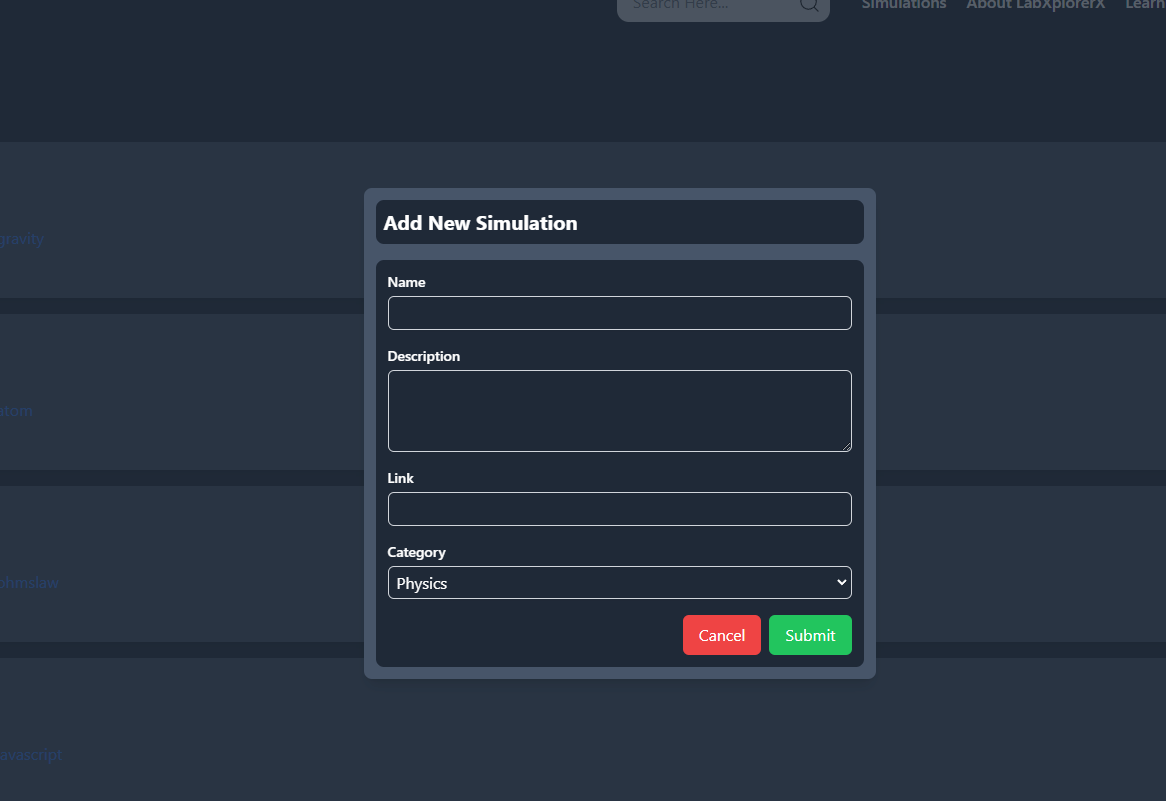
\includegraphics[width = 15cm]{Diagrams/output/addsimulations.png}
    \caption{Add Simulations}
\end{figure}

% Profile Screen
\textbf{Profile Screen:} Below is the screenshot of the Profile Screen, where users can view and edit their profile information.
\begin{figure}[H]
    \centering
    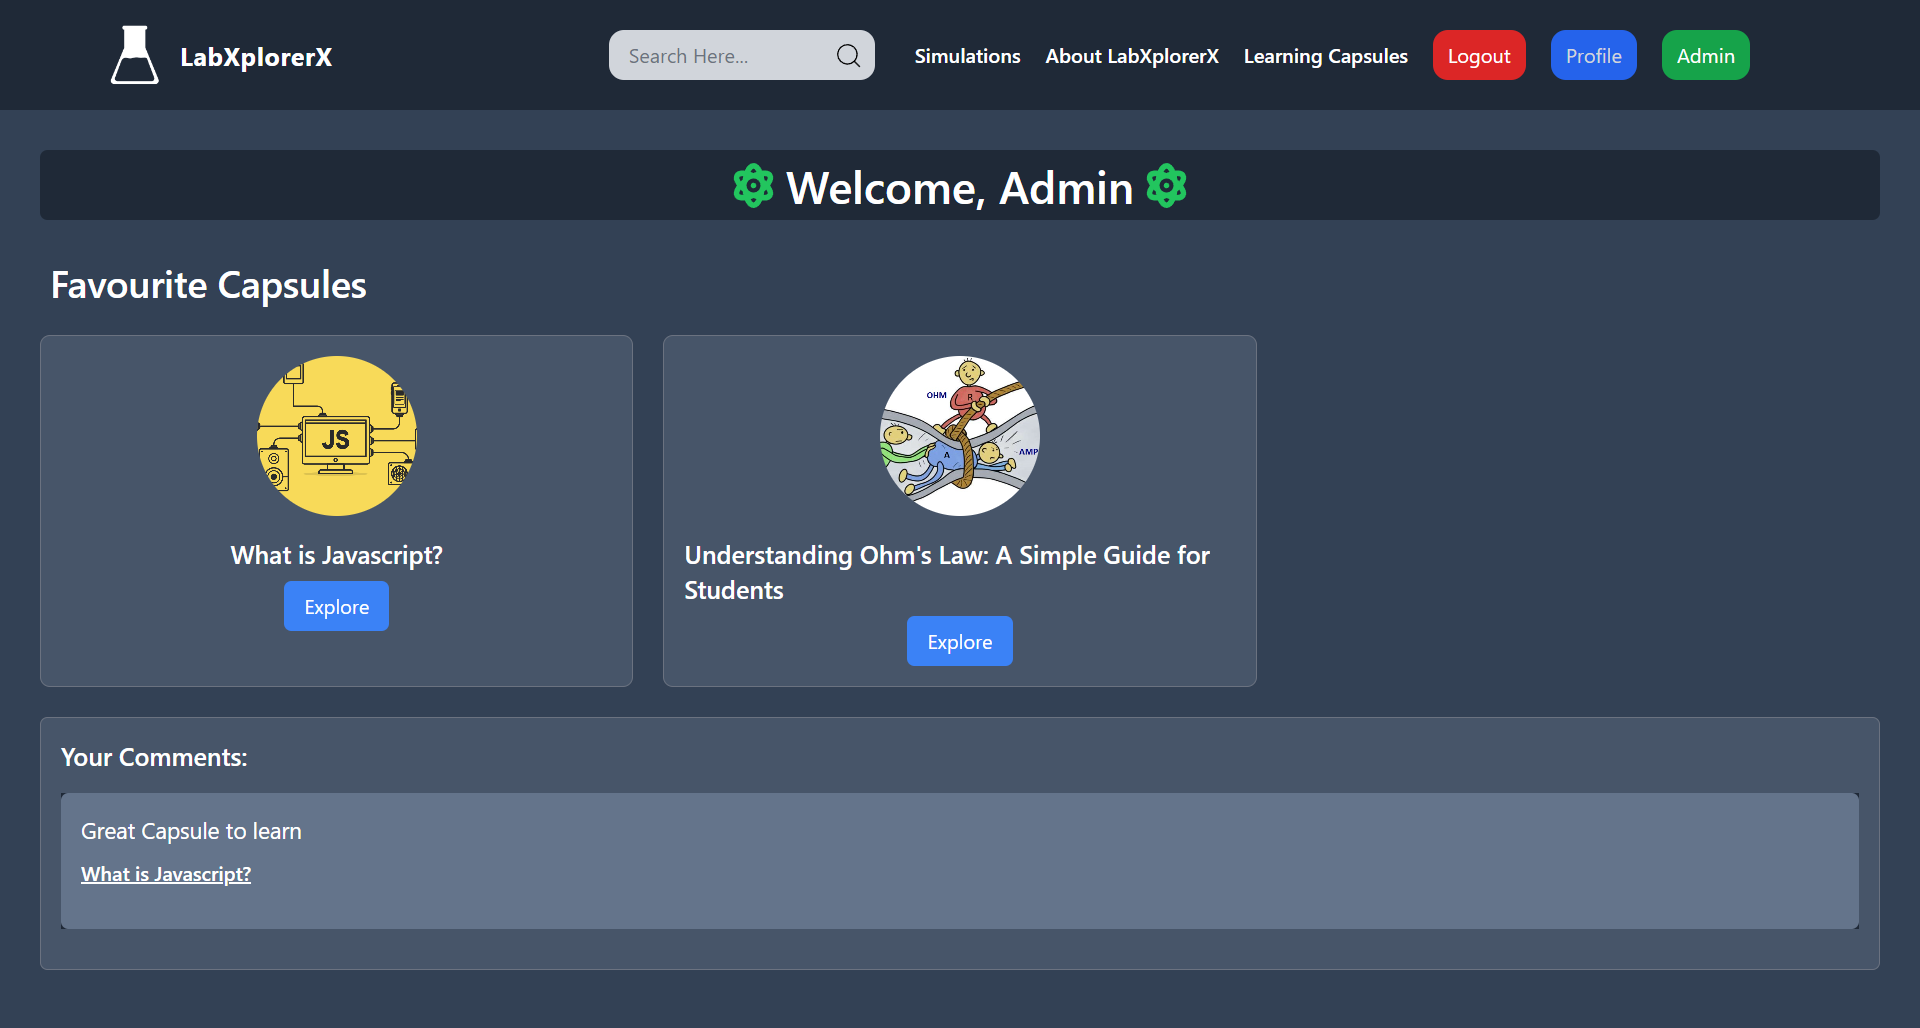
\includegraphics[width = 15cm]{Diagrams/output/profile.png}
    \caption{Profile}
\end{figure}

% Edit Quizzes Screen
\textbf{Edit Quizzes Screen:} Below is the screenshot of the Edit Quizzes Screen, used for creating, updating, and deleting quizzes.
\begin{figure}[H]
    \centering
    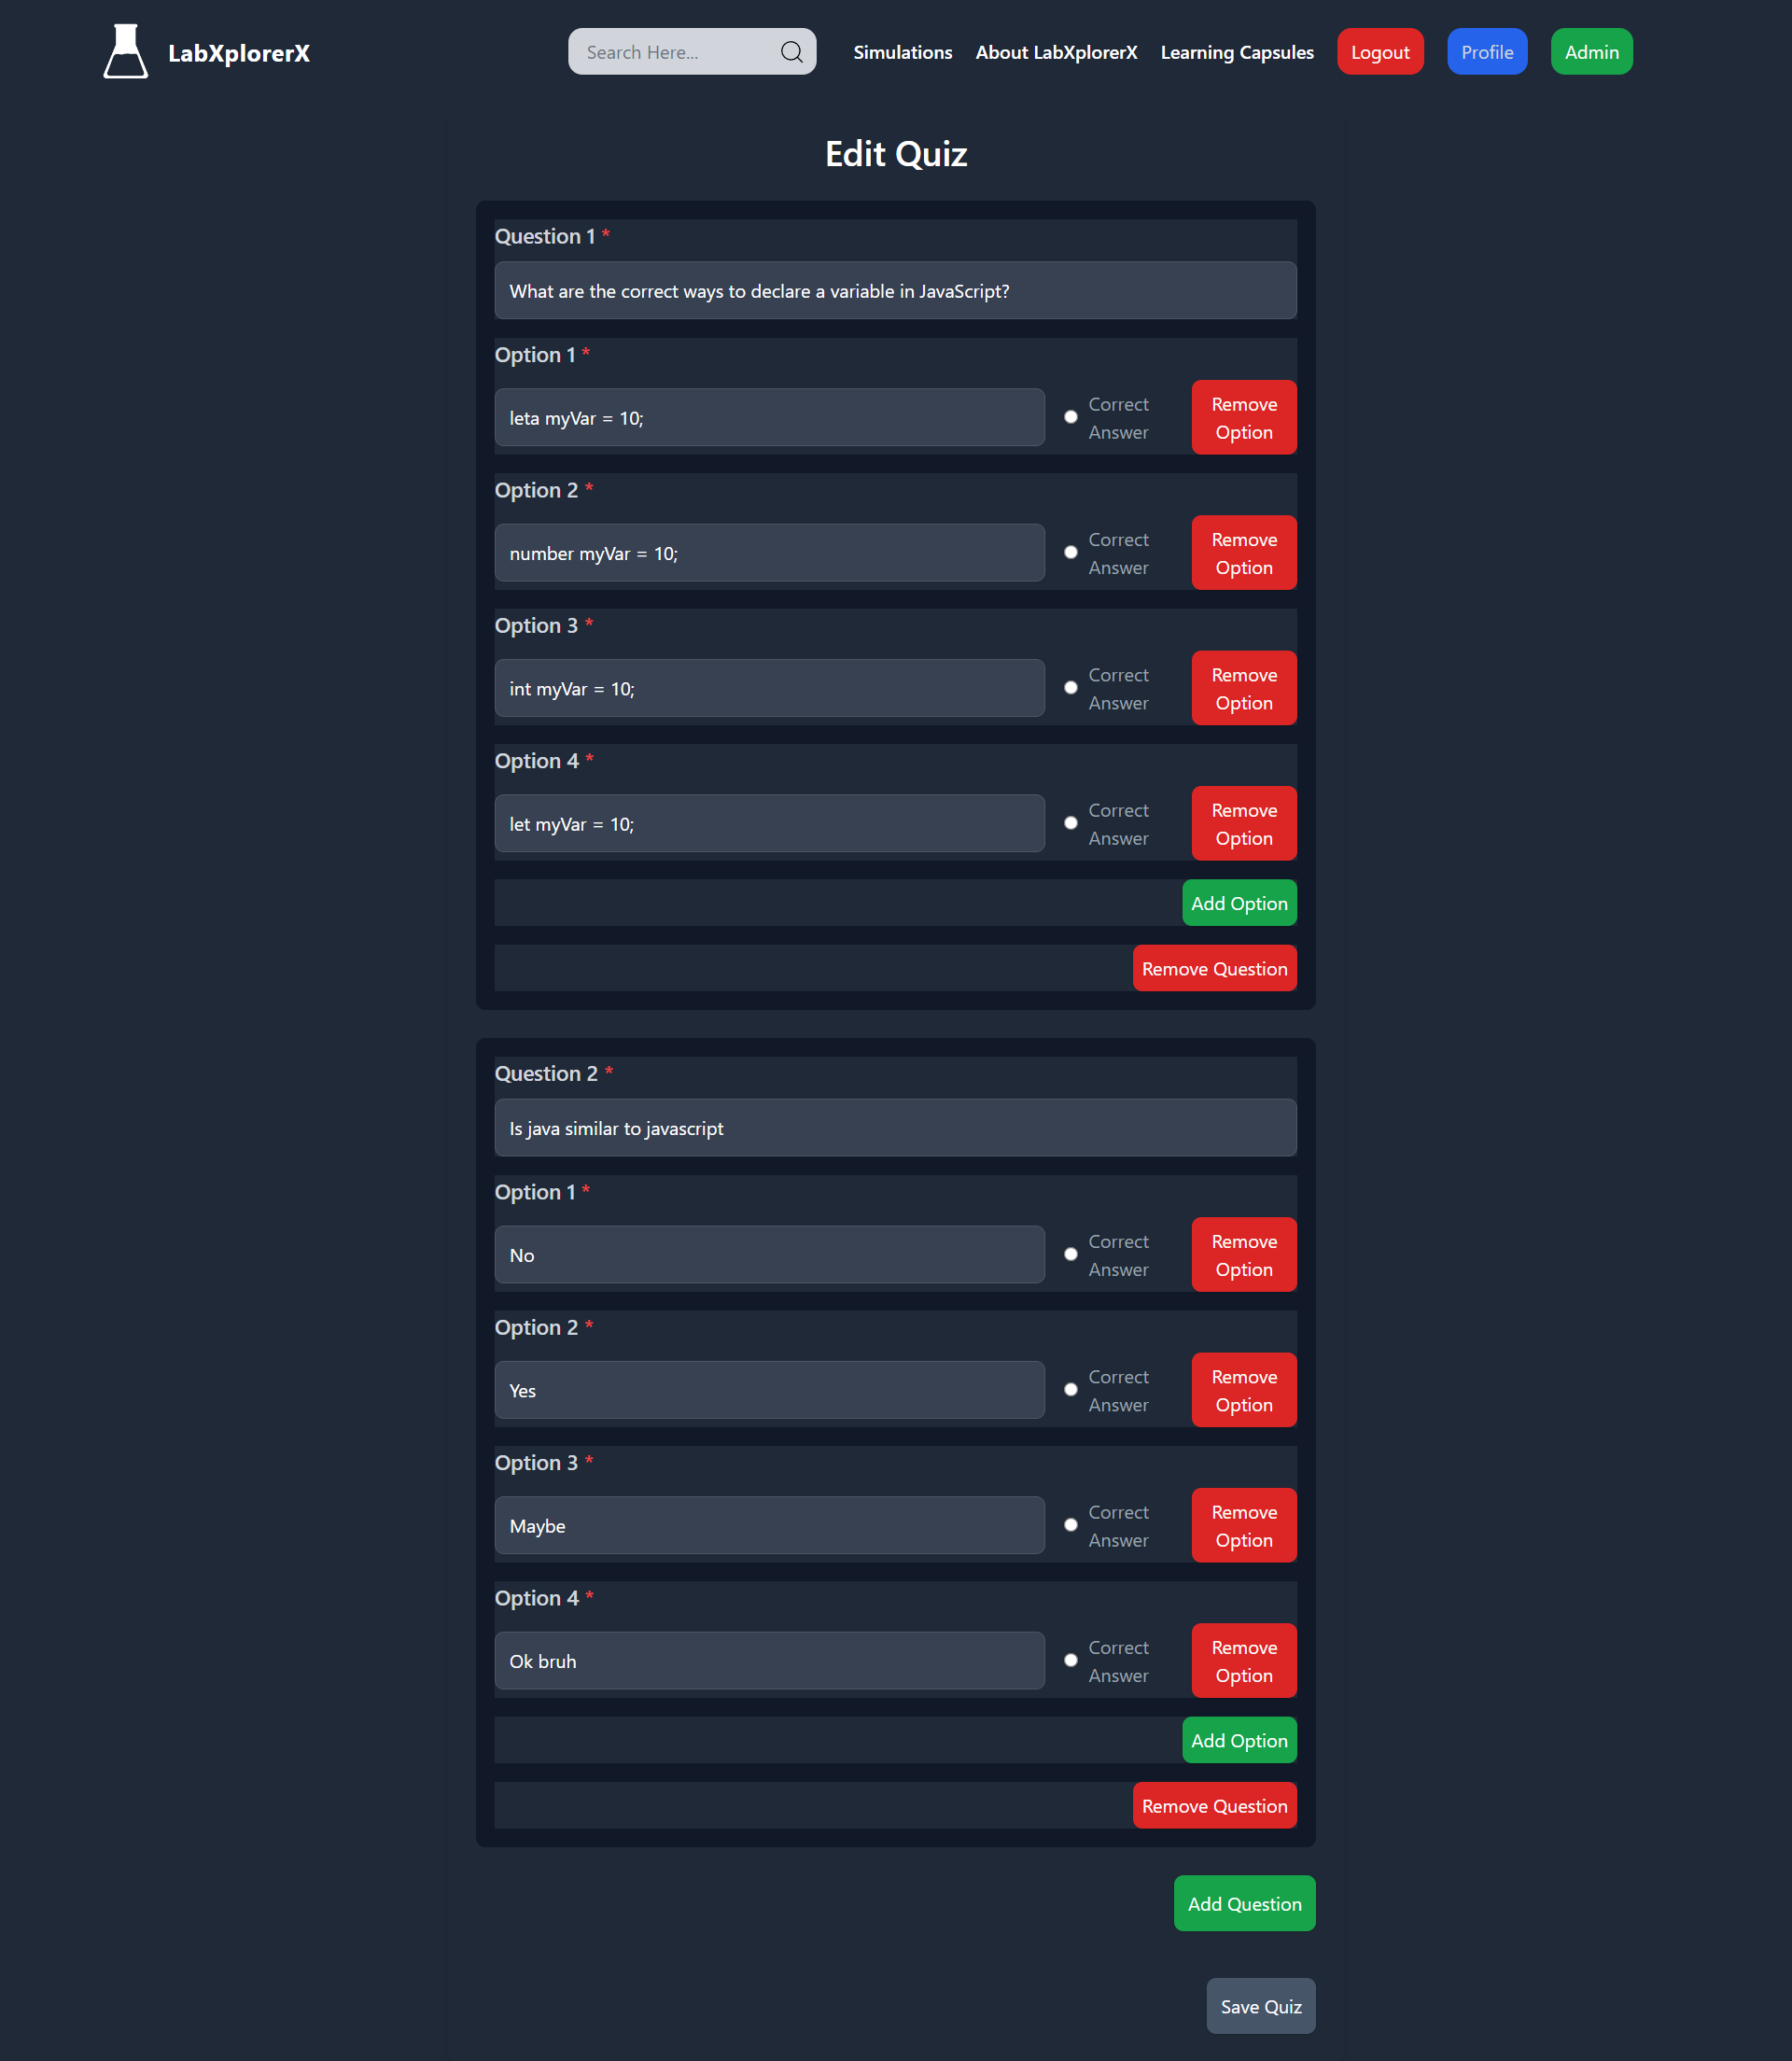
\includegraphics[width = 16cm]{Diagrams/output/edit_quiz.png}
    \caption{CRUD Quizzes}
\end{figure}
\newpage

% Search Results Screen
\textbf{Search Results Screen:} Below is the screenshot of the Search Results Screen, displaying results from user search queries.
\begin{figure}[H]
    \centering
    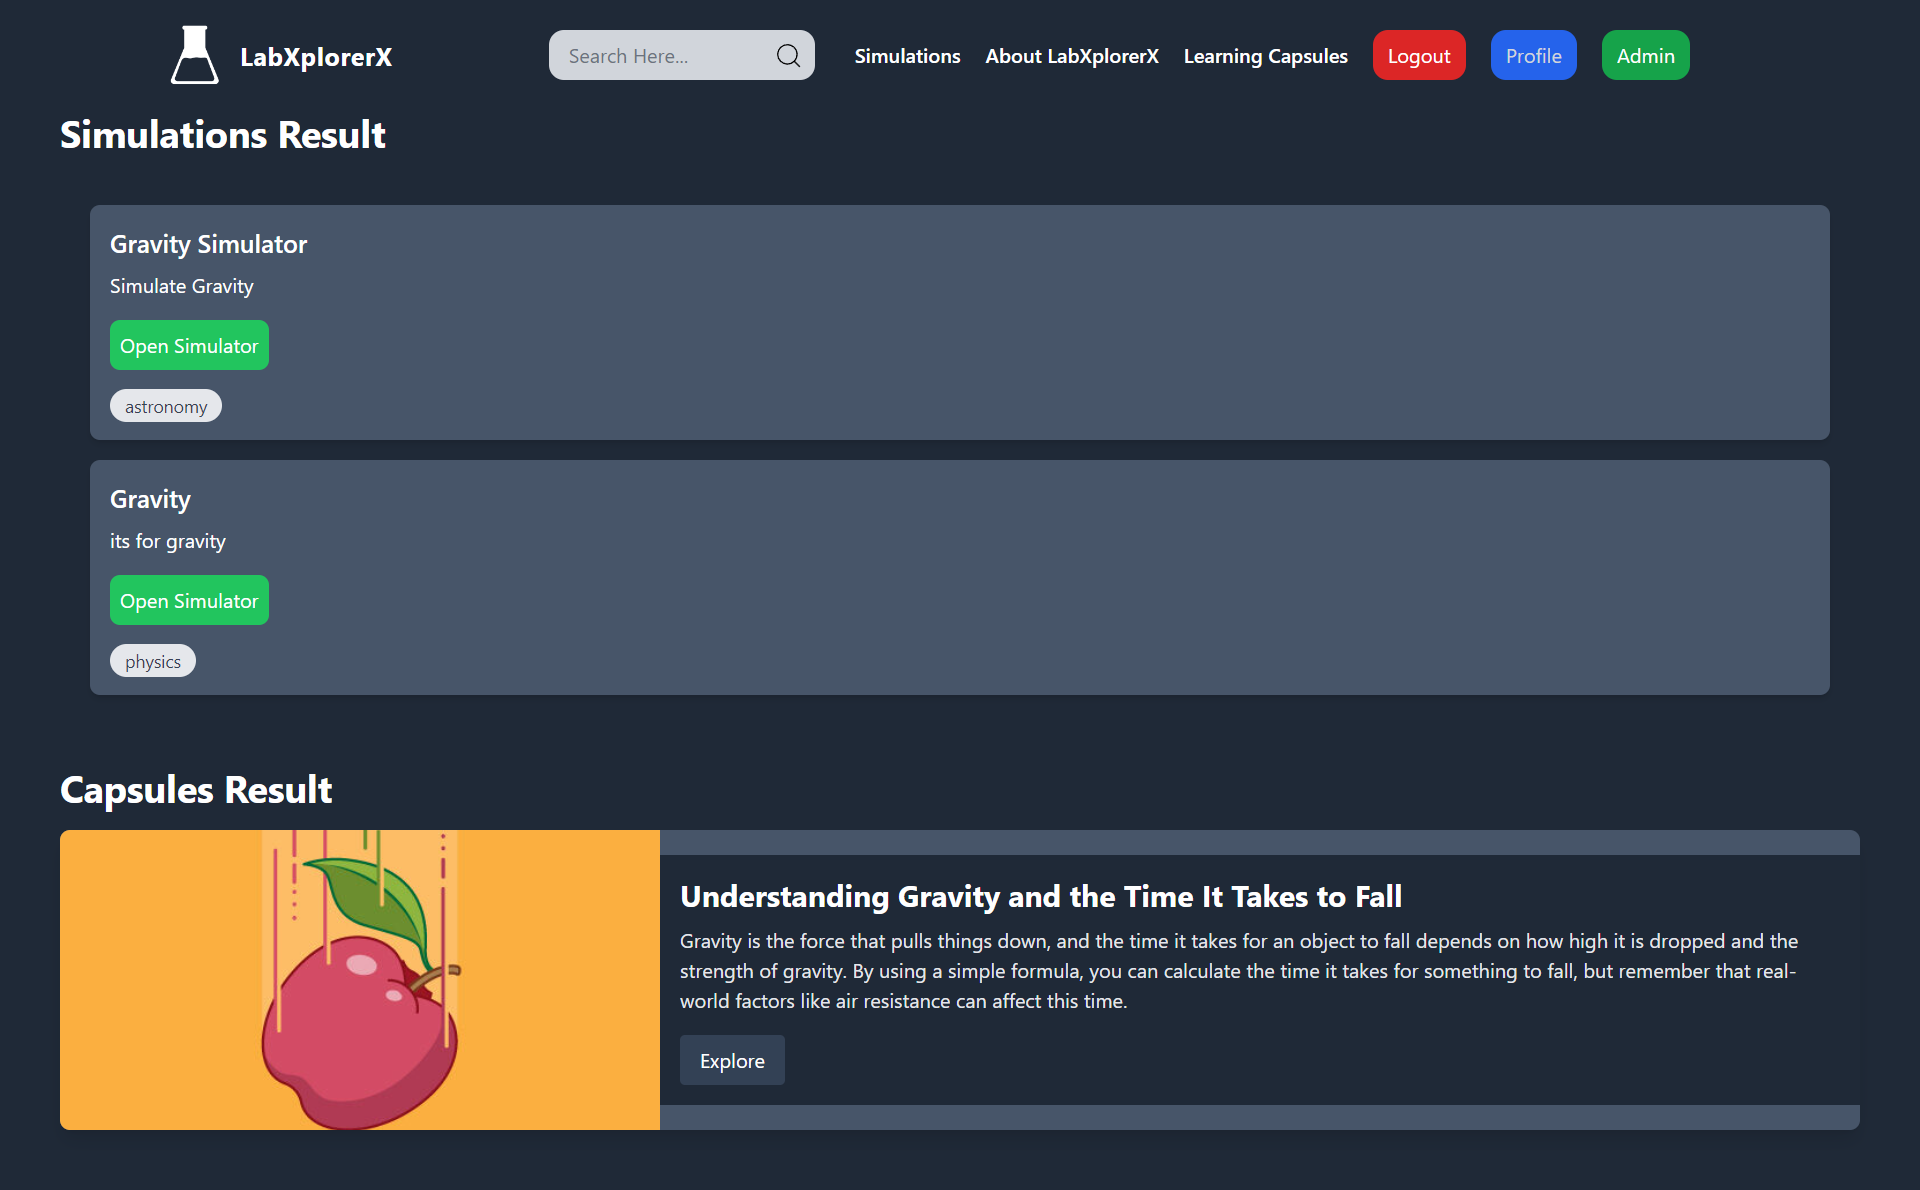
\includegraphics[width = 16cm]{Diagrams/output/search_results.png}
    \caption{Search Results}
\end{figure}
\newpage

% Edit Capsule Screen
\textbf{Edit Capsule Screen:} Below is the screenshot of the Edit Capsule Screen, used for modifying details of existing capsules.
\begin{figure}[H]
    \centering
    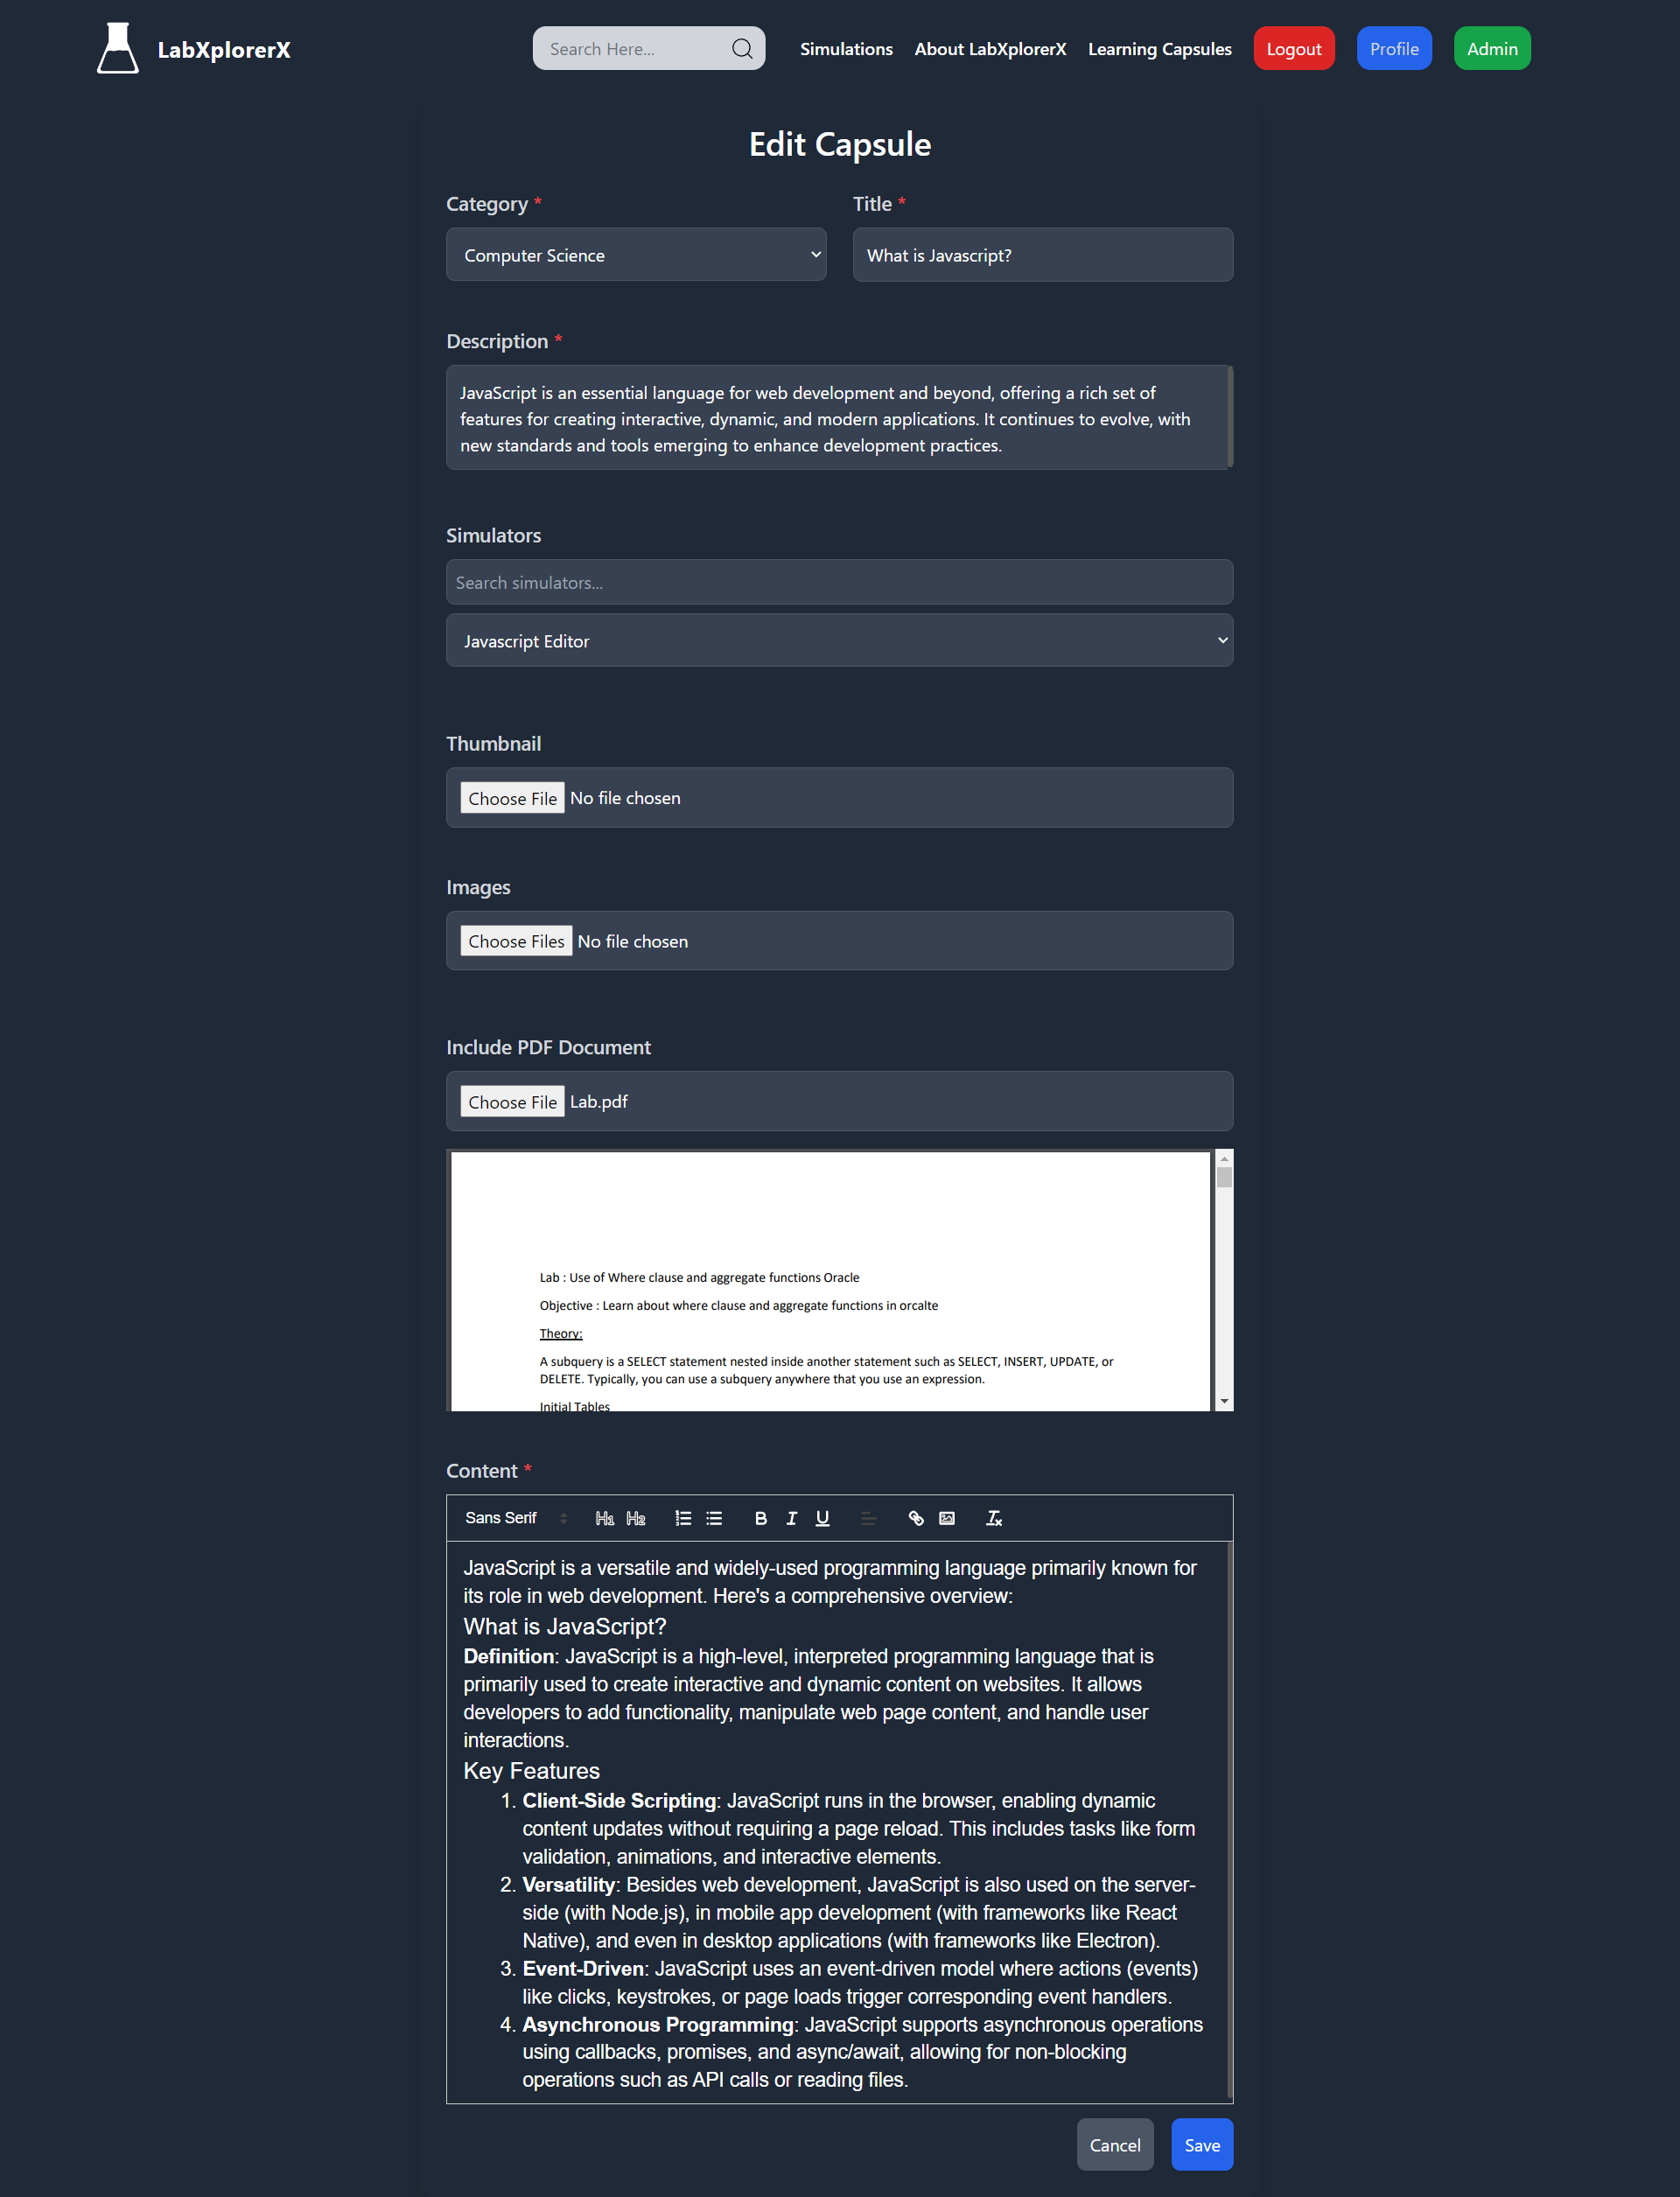
\includegraphics[width = 16cm]{Diagrams/output/edit_capsule.png}
    \caption{Edit Capsule}
\end{figure}

% Add Capsule Screen
\textbf{Add Capsule Screen:} Below is the screenshot of the Add Capsule Screen, where administrators can add new capsules.
\begin{figure}[H]
    \centering
    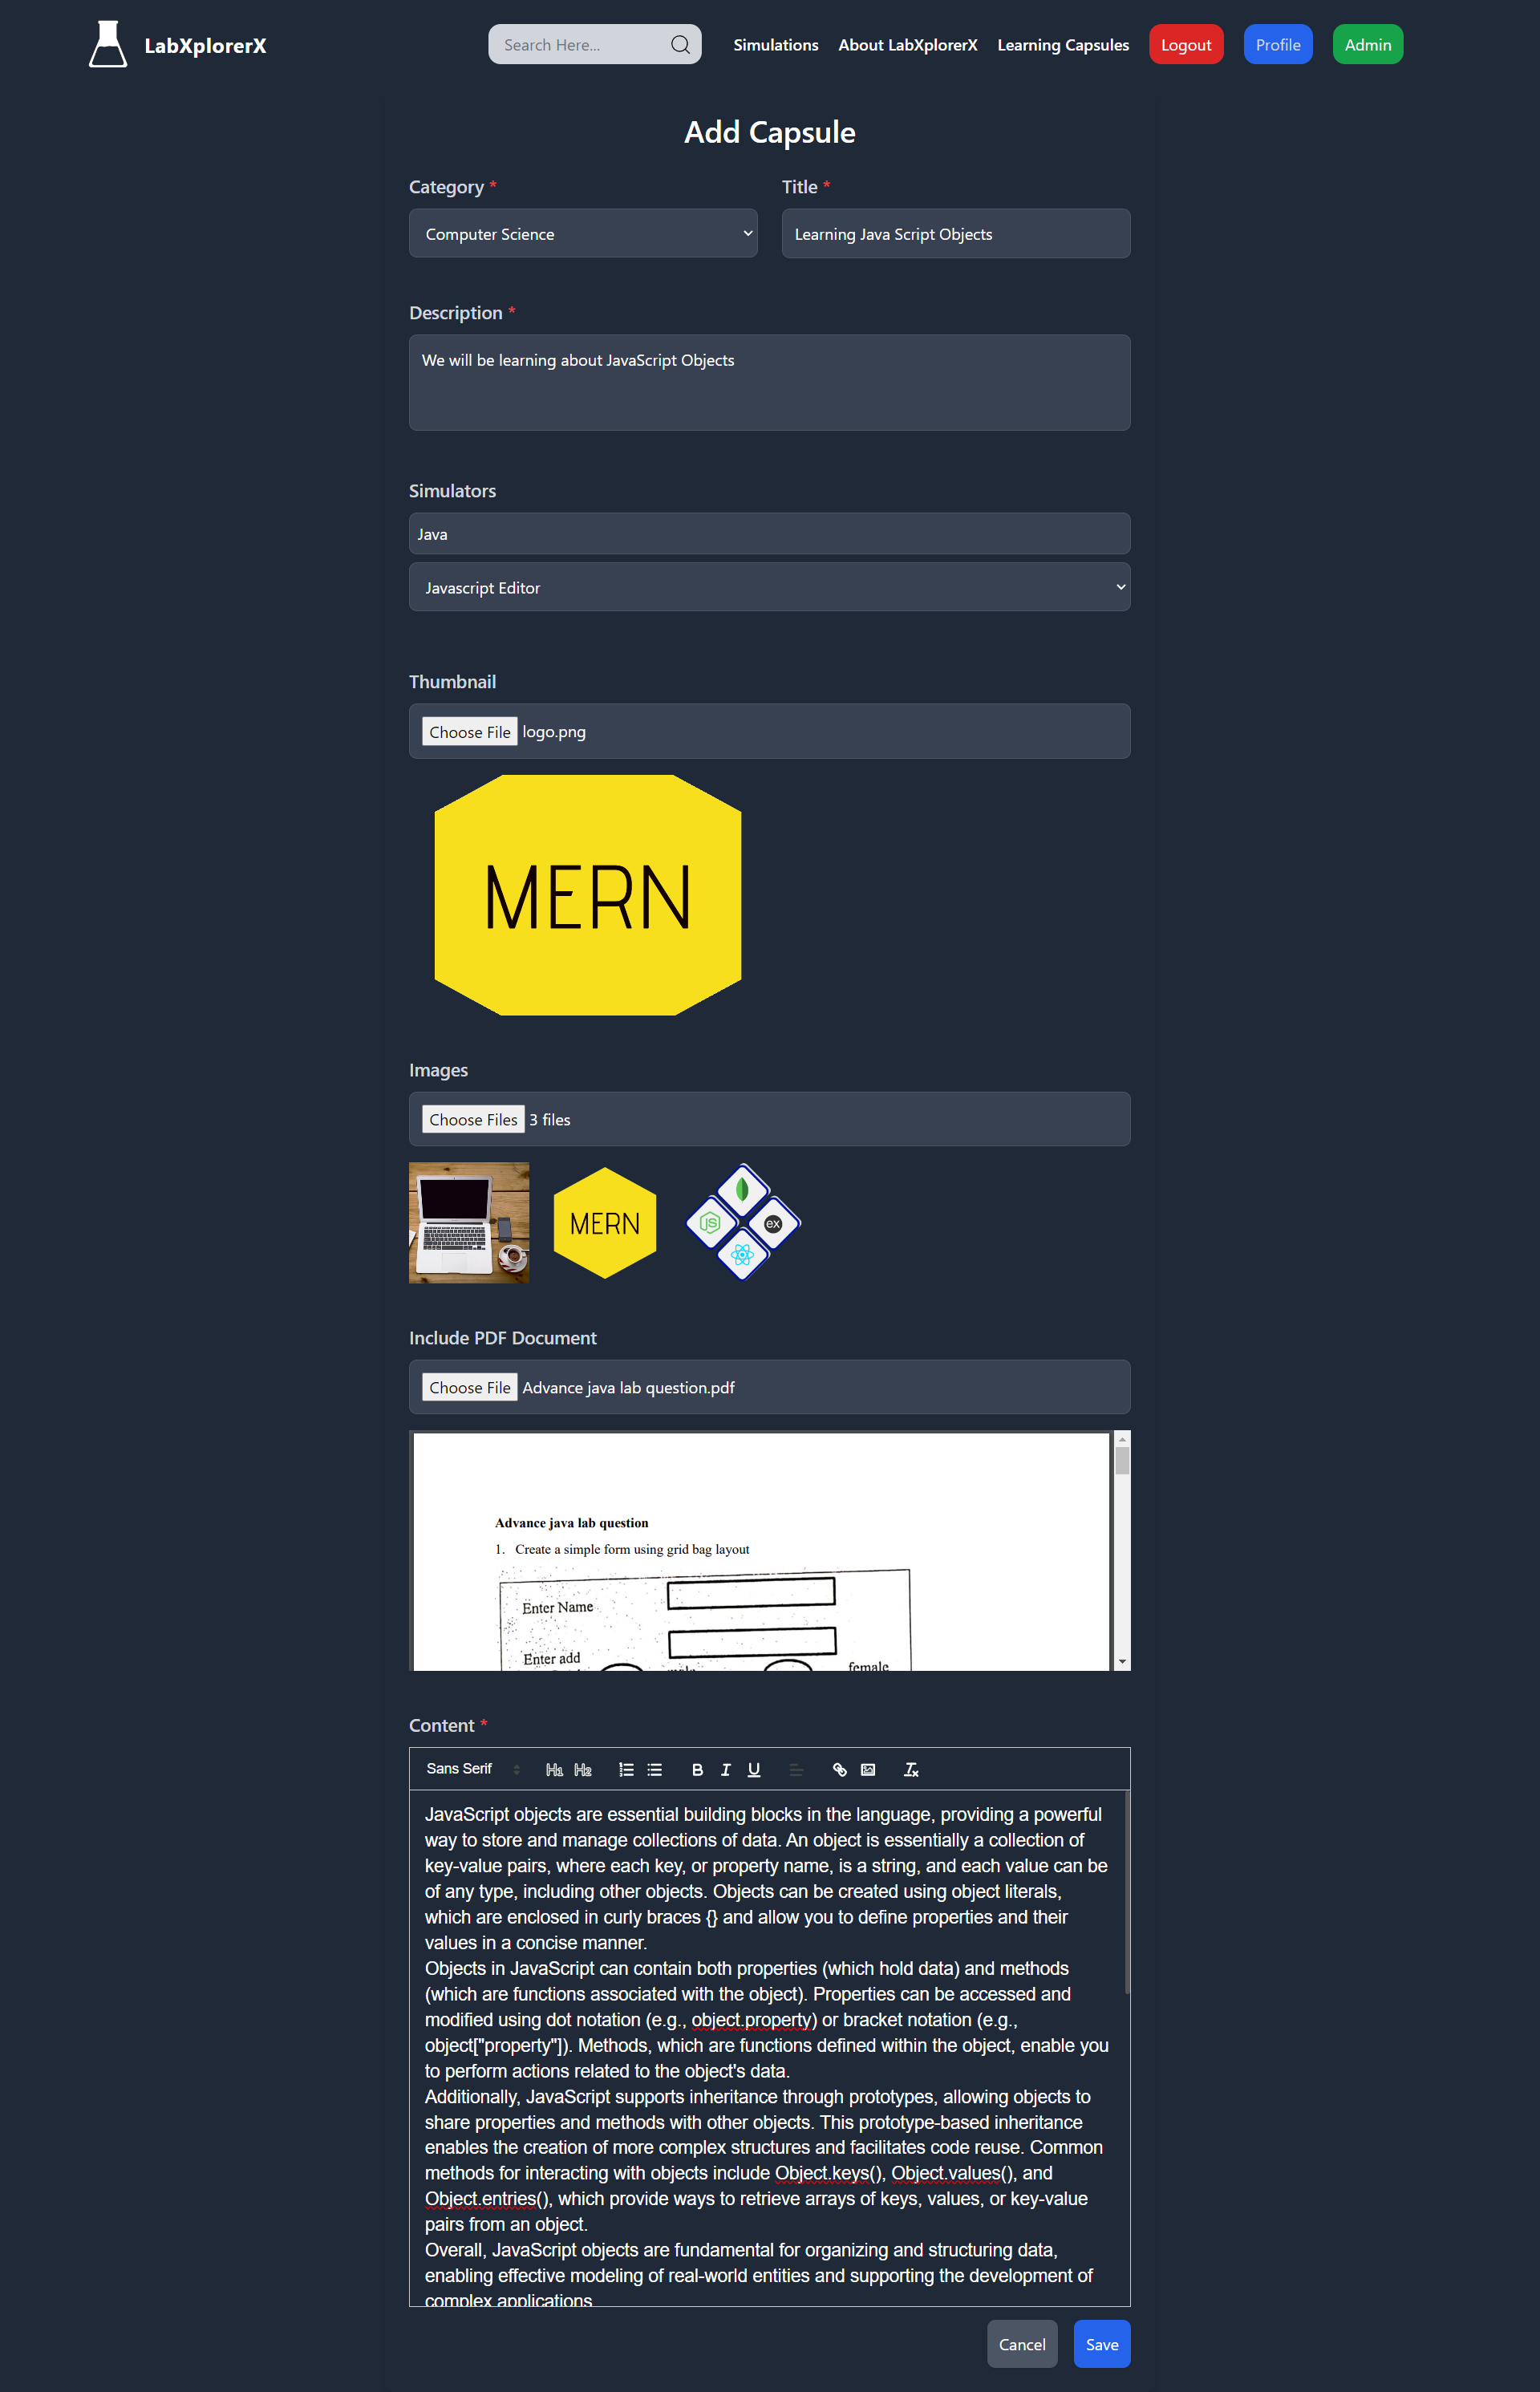
\includegraphics[width = 14cm]{Diagrams/output/addcapsule.png}
    \caption{Add Capsule}
\end{figure}

% After Addition of Capsule Screen
\textbf{After Addition of Capsule Screen:} Below is the screenshot of the screen displayed after a new capsule has been successfully added.
\begin{figure}[H]
    \centering
    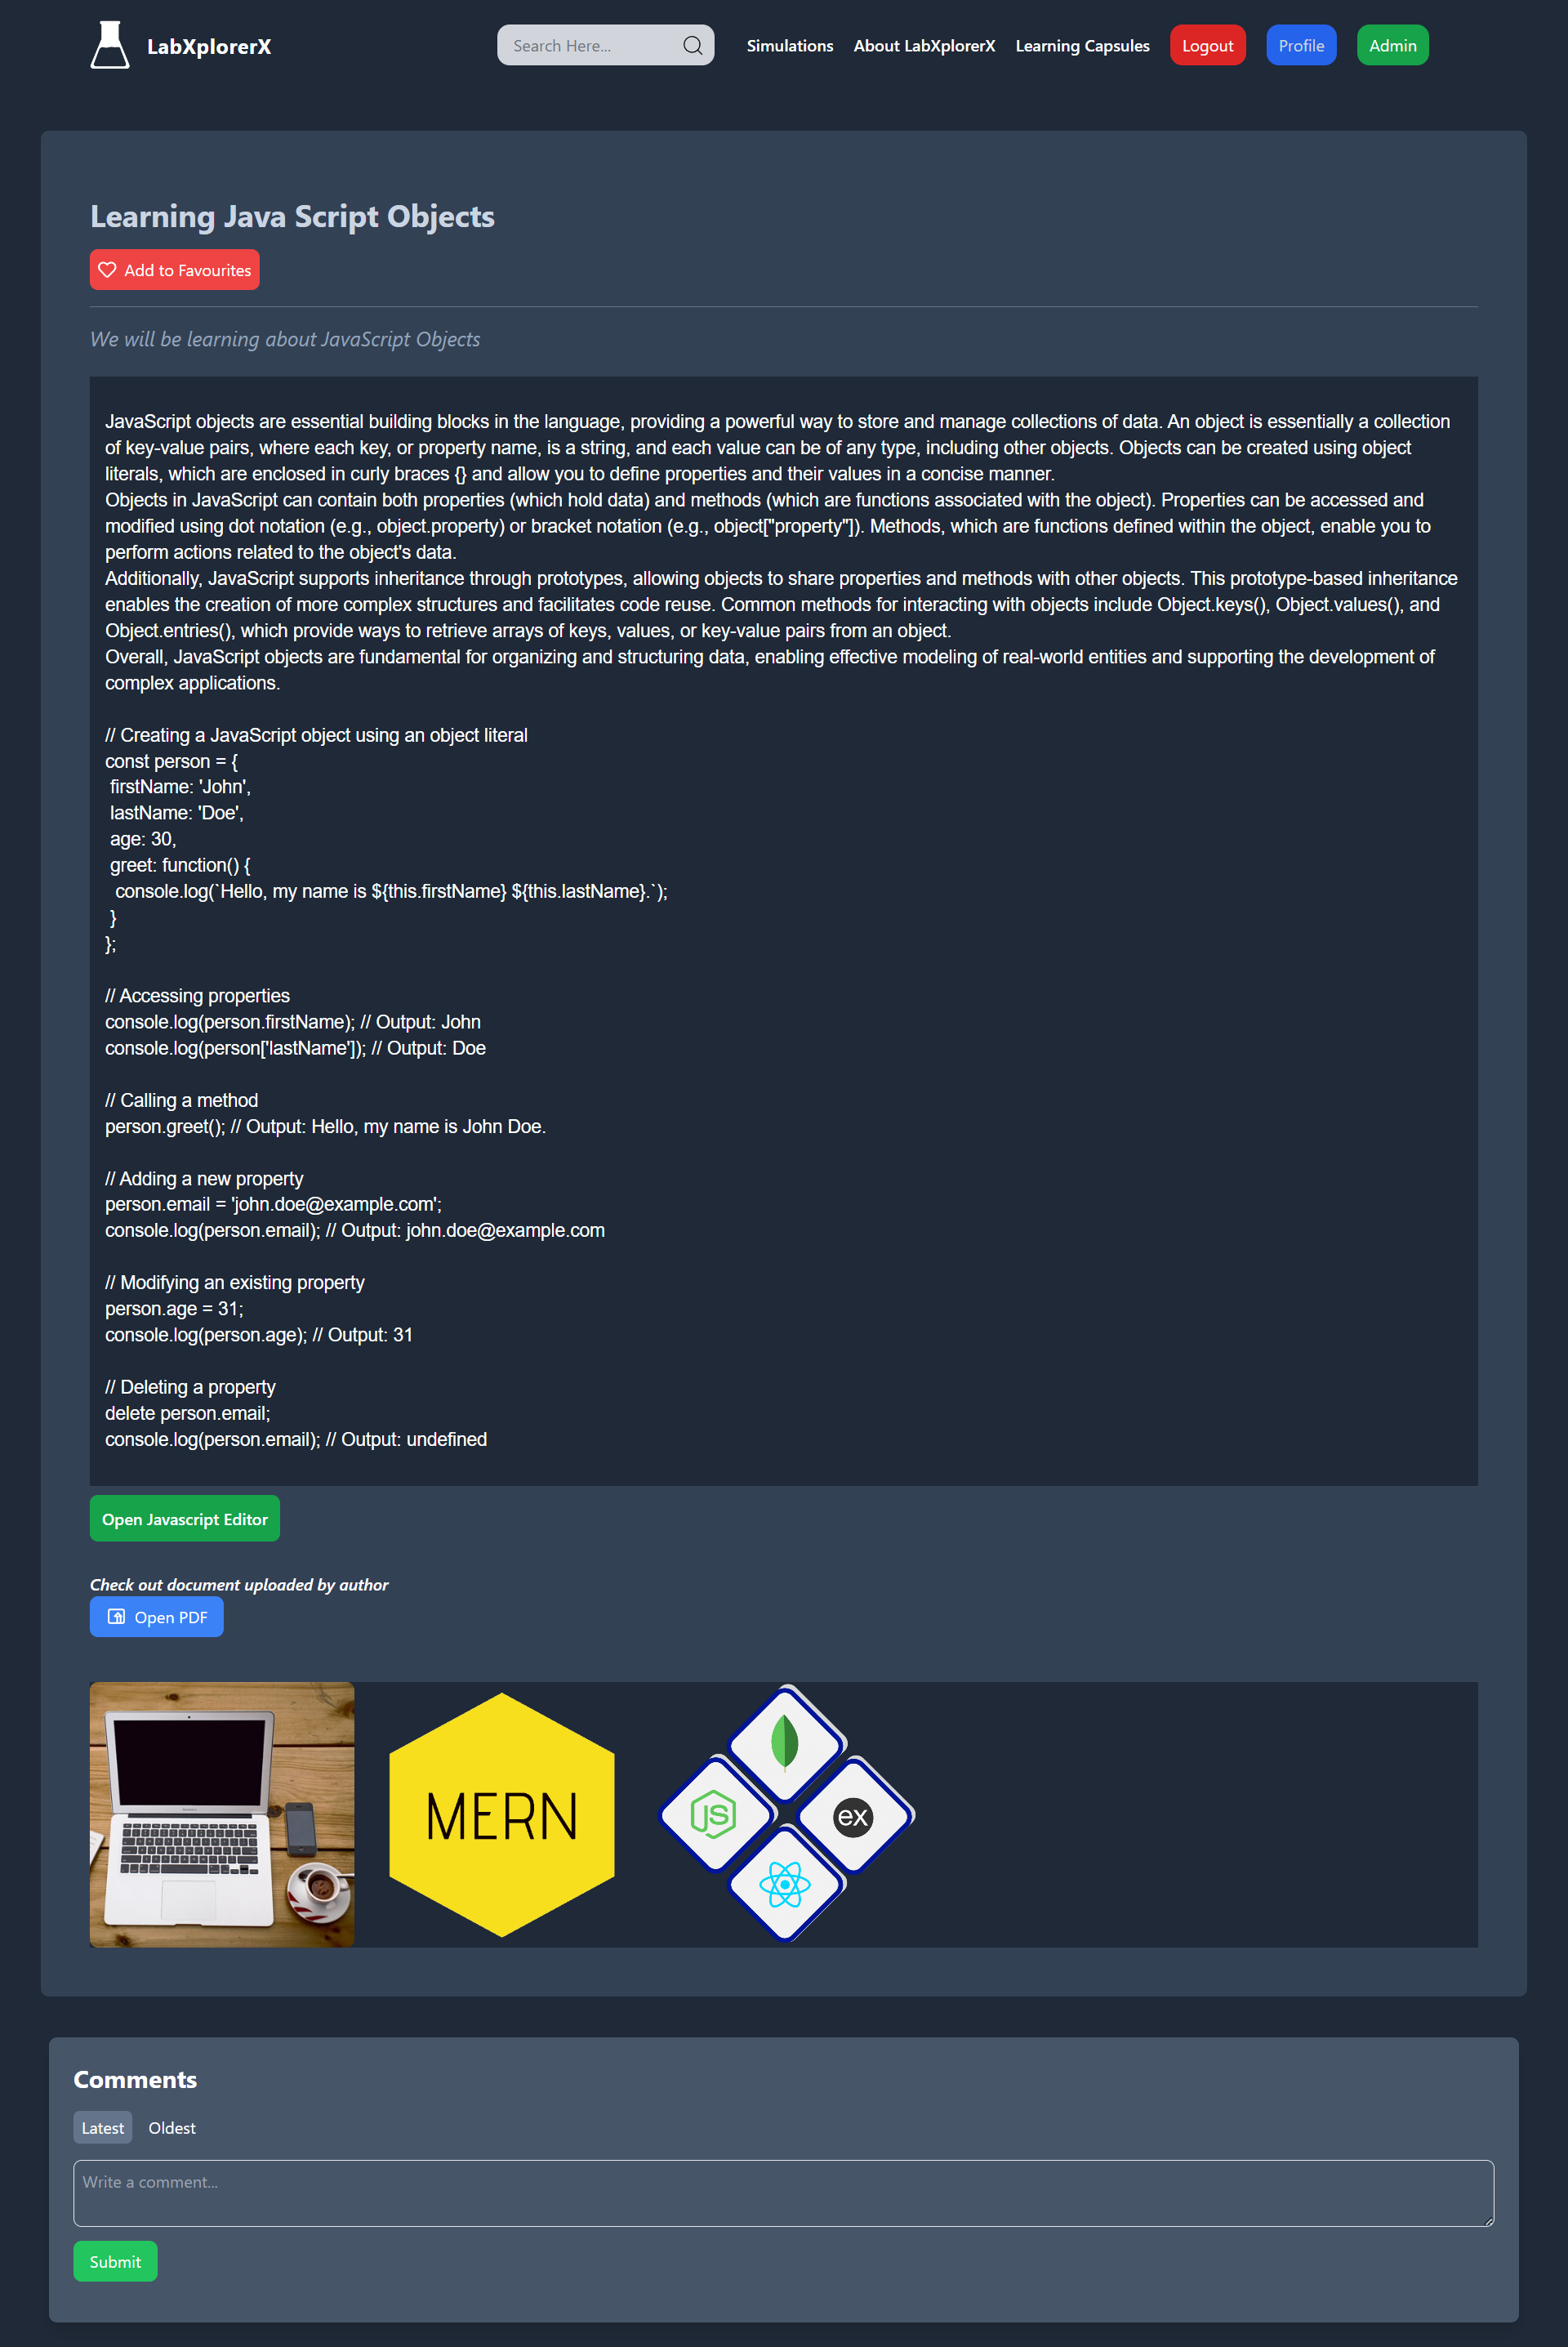
\includegraphics[width = 14cm]{Diagrams/output/after_addition.png}
    \caption{After Addition of Capsule}
\end{figure}

% Gravity Simulator
\textbf{Gravity Simulator:} Below is the screenshot of the Gravity Simulator, demonstrating the principles of gravity.
\begin{figure}[H]
    \centering
    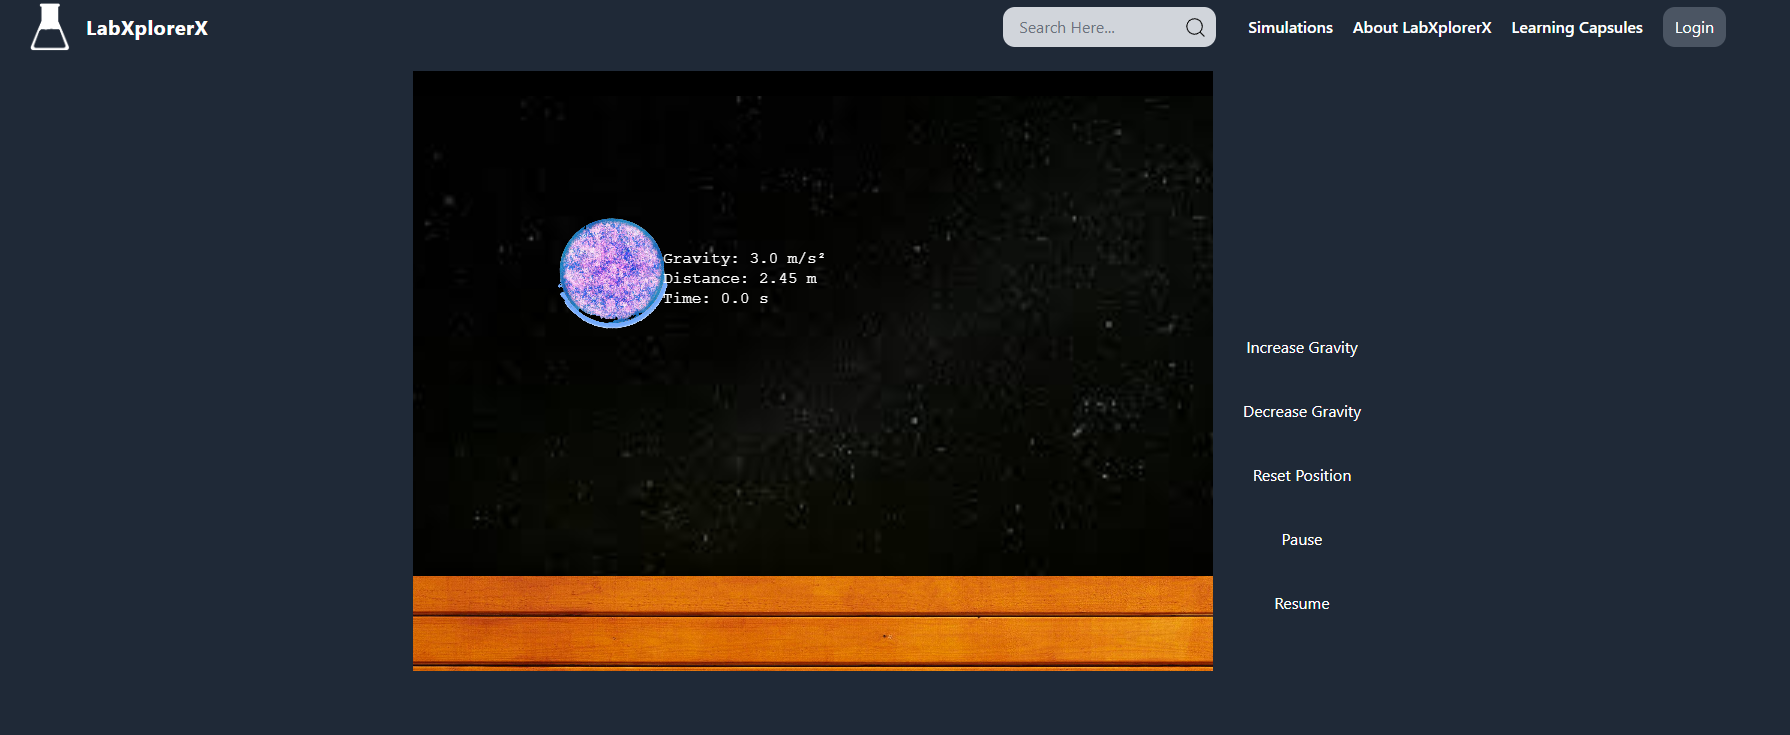
\includegraphics[width = 16cm]{Diagrams/output/gravity.png}
    \caption{Gravity Simulator}
\end{figure}

% Ohm's Law Simulator
\textbf{Ohm's Law Simulator:} Below is the screenshot of the Ohm's Law Simulator, illustrating Ohm's Law in an interactive format.
\begin{figure}[H]
    \centering
    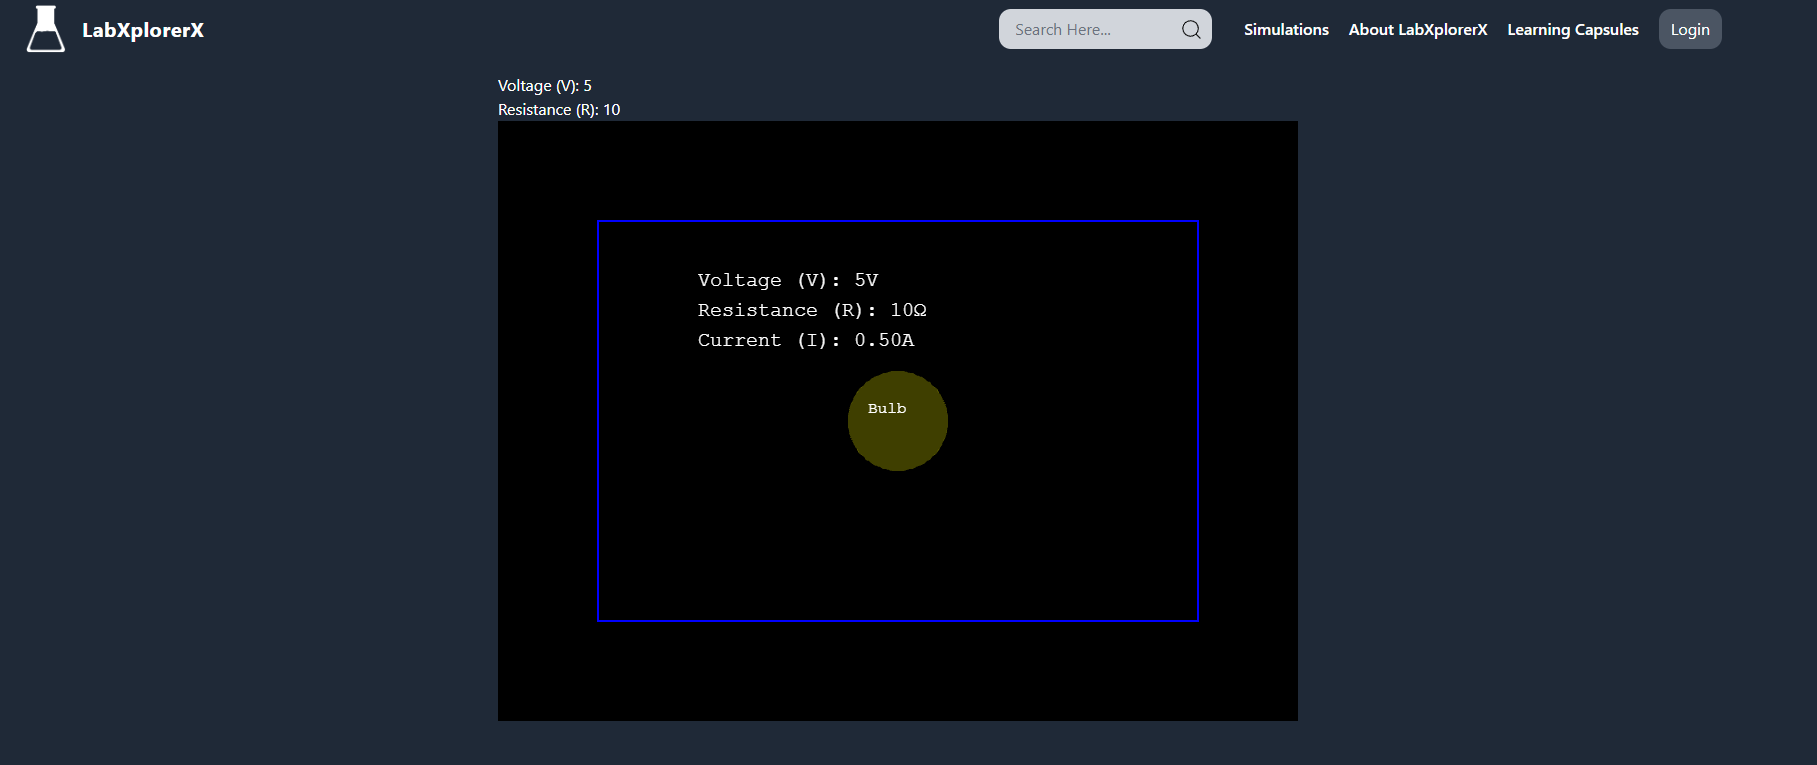
\includegraphics[width = 16cm]{Diagrams/output/ohms.png}
    \caption{Ohm's Law Simulator}
\end{figure}
\newpage

% Atom Simulator
\textbf{Atom Simulator:} Below is the screenshot of the Atom Simulator, allowing users to explore atomic structures.
\begin{figure}[H]
    \centering
    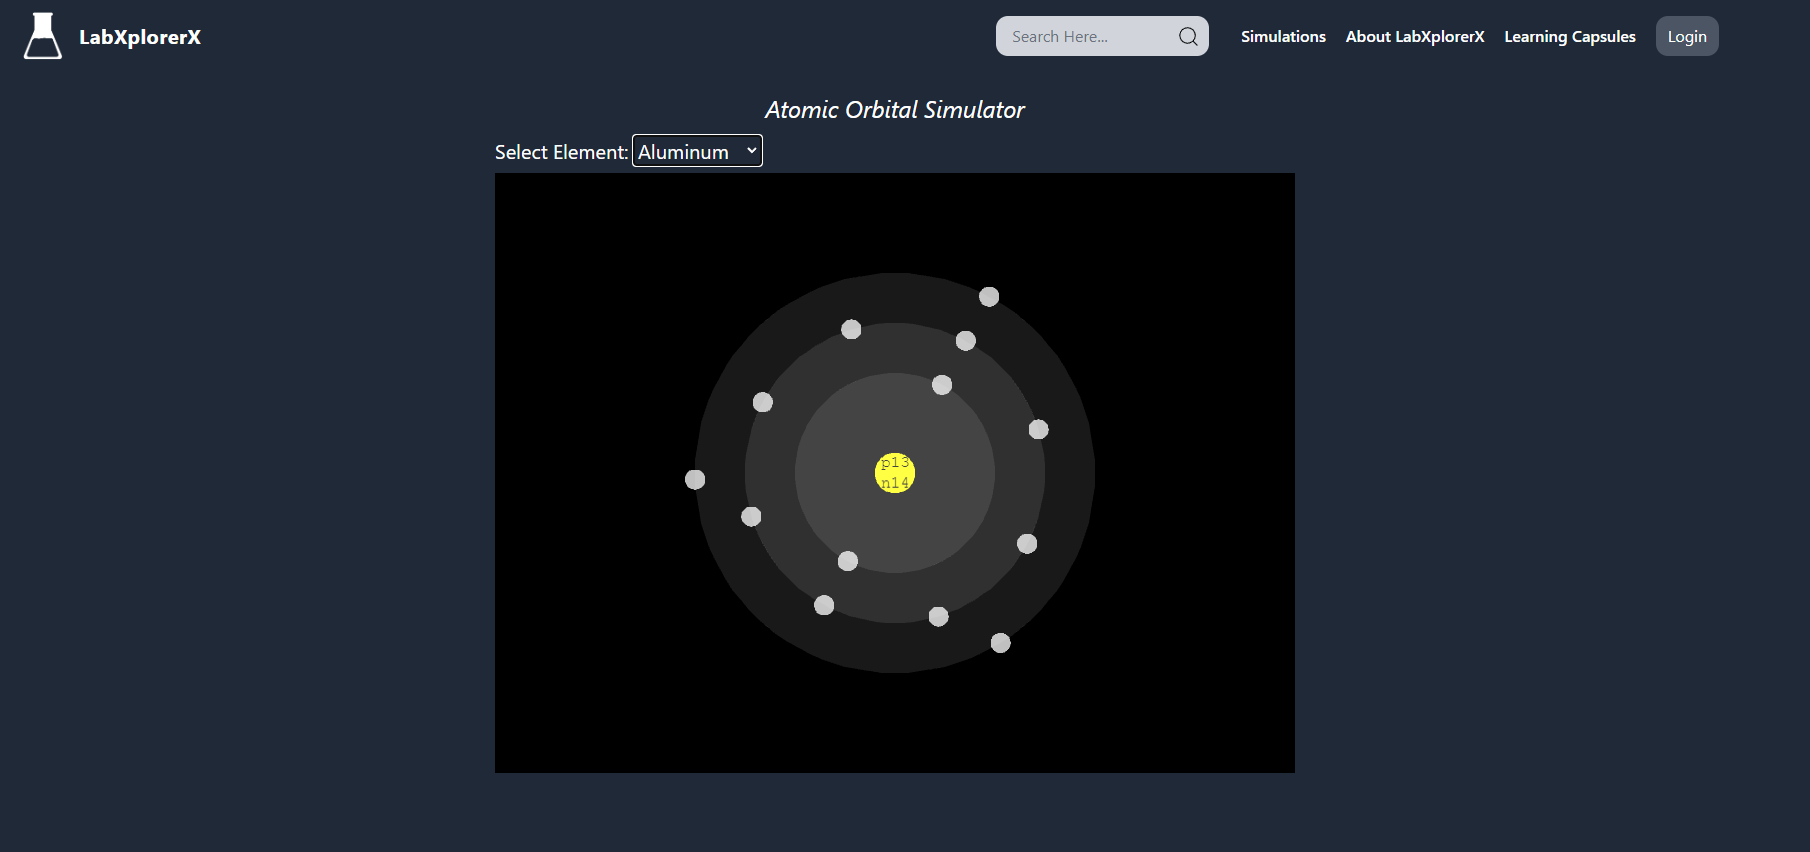
\includegraphics[width = 16cm]{Diagrams/output/atom.png}
    \caption{Atom Simulator}
\end{figure}

% Solar System Simulator
\textbf{Solar System Simulator:} Below is the screenshot of the Solar System Simulator, providing an interactive view of the solar system.
\begin{figure}[H]
    \centering
    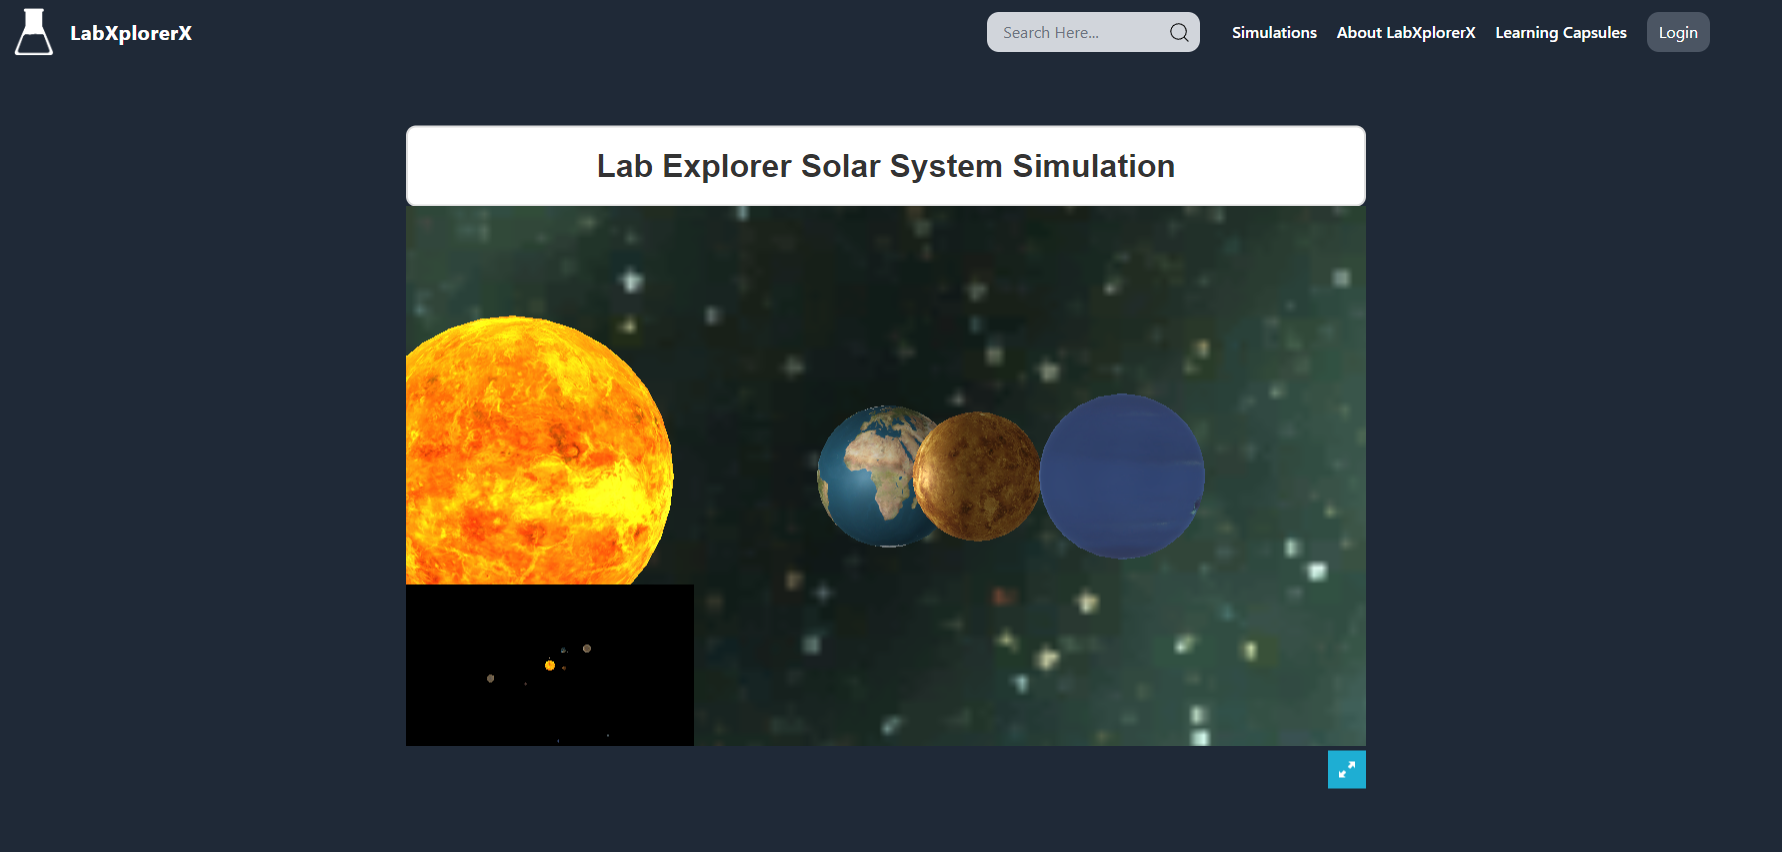
\includegraphics[width = 16cm]{Diagrams/output/solar.png}
    \caption{Solar System Simulator}
\end{figure}
\newpage

% JavaScript Editor
\textbf{JavaScript Editor:} Below is the screenshot of the JavaScript Editor, where users can write and test JavaScript code.
\begin{figure}[H]
    \centering
    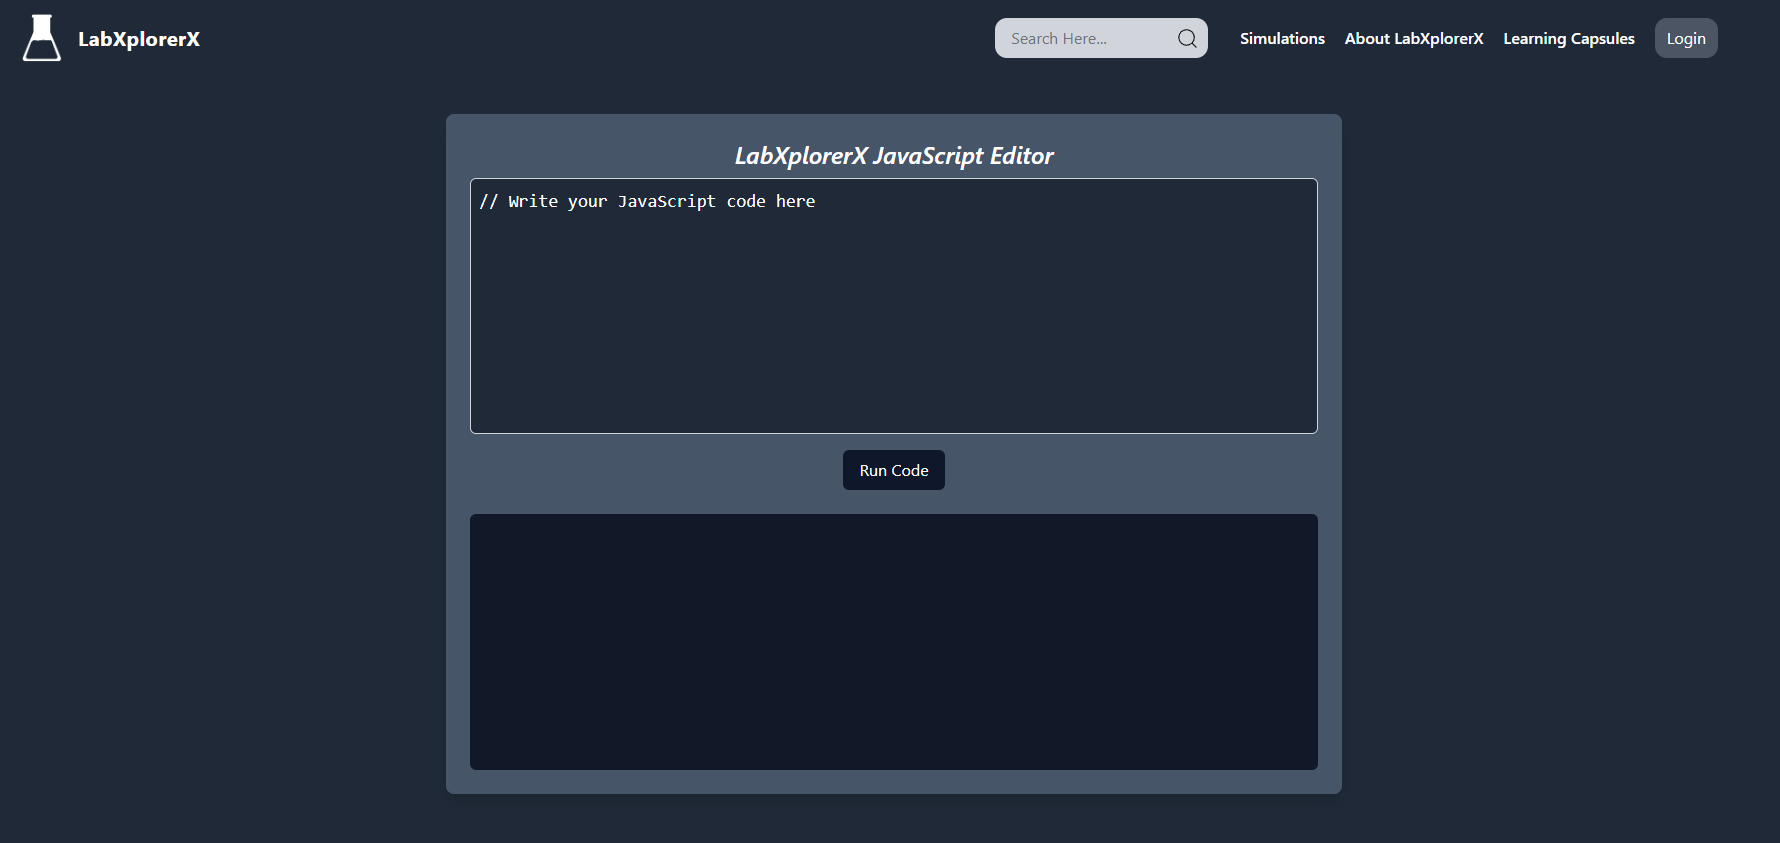
\includegraphics[width = 16cm]{Diagrams/output/js.png}
    \caption{JavaScript Editor}
\end{figure}


\section{Work Remaining}
As the LabXplorerX project progresses, several key tasks remain to be completed. The development team will focus on creating additional simulations to further expand the interactive learning opportunities available to students. The implementation of user profiles is also pending, which will enable students to personalize their learning experience, track progress, and manage their accounts. Additionally, a discussion forum needs to be integrated into the platform, allowing students and teachers to engage in meaningful conversations, share ideas, and collaborate on learning activities.

\begin{itemize}[leftmargin=1cm]
    \item \textbf{More Simulations:} Continue creating additional simulations to broaden the range of interactive learning experiences available to students.
    
    \item \textbf{User Profiles:} Implement personalized user profiles, enabling students to track their progress, manage their accounts, and enhance their learning experience.
    
    \item \textbf{Discussion Forum:} Develop and integrate a discussion forum, facilitating communication and collaboration between students and teachers within the platform.
\end{itemize}